\documentclass[11pt,a4paper]{book}
% \usepackage{titlesec}
\usepackage[legalpaper, margin=0.8in]{geometry}
\usepackage[brazil]{babel}
\usepackage[utf8]{inputenc}
\usepackage{xcolor}
\usepackage{listings}
\usepackage{amsmath}
\usepackage{amssymb}
\usepackage{amsfonts}
\usepackage{graphicx}
\usepackage{titling}
\usepackage{caption}
\usepackage{multicol}
\usepackage{paracol}
\usepackage{indentfirst}
\usepackage{tikz}
\usetikzlibrary {graphs,quotes}
\usepackage[colorlinks=true,linkcolor=blue!80!brown!80!red]{hyperref}
\renewcommand{\thechapter}{\Roman{chapter}}
\renewcommand{\thesection}{\arabic{chapter}.\arabic{section}}
\renewcommand{\mod}[1]{\;\left(\bmod\; #1\right)}
\newcommand\tab[1][0.5cm]{\hspace*{#1}}
\newread\hashfile
\newcommand{\hashlineid}[1]{%
  \ifnum#1<10 00#1\else\ifnum#1<100 0#1\else#1\fi\fi
}
\newcommand{\hashlookup}[1]{%
  \ifcsname hashline\number\numexpr#1\relax\endcsname
    \csname hashline\number\numexpr#1\relax\endcsname
  \fi
}
\newcommand{\hashnumberstyle}[1]{%
  \scriptsize\color{black}\ttfamily\makebox[8.2em][r]{\hashlineid{#1} \hashlookup{#1}}%
}
\newcommand{\readhashline}[1]{%
  \expandafter\parsehashline#1 \relax
}
\def\parsehashline#1 #2\relax{%
  \def\hashindex{#1}%
  \def\hashvalue{#2}%
  \def\hashalllabel{ALL}%
  \ifx\hashindex\hashalllabel
    \def\hashall{#2}%
  \else
    \expandafter\def\csname hashline\number\numexpr#1\relax\endcsname{#2}%
  \fi
}
\newcommand{\loadhashes}[1]{%
  \def\hashall{}%
  \openin\hashfile=#1.hash
  \loop
    \read\hashfile to \hashline
    \ifeof\hashfile\else
    \readhashline{\hashline}%
  \repeat
  \closein\hashfile
}
\newcommand{\inputwithhash}[1]{%
  \noindent
  \begingroup
  \loadhashes{#1}
  \lstinputlisting[
    basicstyle=\ttfamily\footnotesize,
    numberstyle=\hashnumberstyle,
    xleftmargin=2.4em,
    numbersep=3pt
  ]{#1}
  \noindent\hspace*{5.2em}\llap{\scriptsize\color{black}\ttfamily\makebox[8.2em][r]{ALL \hashall}\kern3pt}\par
  \endgroup
}
\usepackage{tocloft}

\addtolength{\cftchapnumwidth}{15pt}


\definecolor{mygreen}{rgb}{0.1,0.1,1.0}
\definecolor{mygray}{rgb}{0.5,0.5,0.5}
\definecolor{mymauve}{rgb}{0.58,0,0.82}
\lstset{ 
  backgroundcolor=\color{white},   % choose the background color; you must add \usepackage{color} or \usepackage{xcolor}; should come as last argument
  basicstyle=\ttfamily,        % the size of the fonts that are used for the code
  breakatwhitespace=false,         % sets if automatic breaks should only happen at whitespace
  breaklines=true,                 % sets automatic line breaking
  captionpos=b,                    % sets the caption-position to bottom
  commentstyle=\color{mygreen},    % comment style
  deletekeywords={...},            % if you want to delete keywords from the given language
  escapeinside={\%*}{*)},          % if you want to add LaTeX within your code
  extendedchars=false,              % lets you use non-ASCII characters; for 8-bits encodings only, does not work with UTF-8
  firstnumber=1,                % start line enumeration with line 1000
  frame=single,	                   % adds a frame around the code
  keepspaces=true,                 % keeps spaces in text, useful for keeping indentation of code (possibly needs columns=flexible)
  keywordstyle=\color{blue},       % keyword style
  language=C++,                 % the language of the code
  morekeywords={*,...},            % if you want to add more keywords to the set
  numbers=left,                    % where to put the line-numbers; possible values are (none, left, right)
  numbersep=5pt,                   % how far the line-numbers are from the code
  numberstyle=\tiny\color{mygray}, % the style that is used for the line-numbers
  rulecolor=\color{black},         % if not set, the frame-color may be changed on line-breaks within not-black text (e.g. comments (green here))
  showspaces=false,                % show spaces everywhere adding particular underscores; it overrides 'showstringspaces'
  showstringspaces=false,          % underline spaces within strings only
  showtabs=false,                  % show tabs within strings adding particular underscores
  stepnumber=1,                    % the step between two line-numbers. If it's 1, each line will be numbered
  stringstyle=\color{mymauve},     % string literal style
  tabsize=2,	                   % sets default tabsize to 2 spaces \lstinputlisting; also try caption instead of title
}
% \title{Monkeys LIB 2.0\\ Guadalajara Edition}

% \subtitle{Guadalajara Edition}
\author{Monkeys}
\date{2025}

\begin{document}
\begin{titlingpage} %This starts the title page
\begin{center}

\includegraphics[width=5cm]{monkeys vazado azul.png}\\ %Put the logo you want here
\vspace{8cm} %You can control the vertical distance
\begin{huge} 
\textbf{Monkeys LIB 5.0} \\
\theauthor\\
\end{huge}
\vspace{12cm} %Put the distance you need.

\includegraphics[width=5.5cm]{UFG_LOGO.png}\\ %Put the logo you want here
\begin{LARGE}
\thedate
\end{LARGE}
\end{center}
\end{titlingpage}
 
 % https://www.overleaf.com/7646931546nfyjyscbbjjm
{\fontsize{40}{48} \selectfont }
\tableofcontents{}
\chapter{Início}
      \section{Autores}

    As vezes, dizer obrigado é importante, esse livro tem o nome e o coração de um grupo, cheio de discordâncias. Nós somos \textbf{diferentes} e isso é o que nos faz \textbf{fortes}. Acredite em si mesmo, e se você não consegue, acredite nas pessoas ao seu lado.

    Obrigado.

    Aqui uma lista de nomes que contribuíram com esse livro (para aqueles que estão se perguntando, isso foi ordenado usando random\_shuffle no C++20 usando srand(252)):
    \begin{itemize}
        \item Lesin
        \item Alunea
        \item Nopebi Lifesa
        \item Atak Kichan
        \item Faslecar
        \item Nollyad
        \item Laelovatsug
        \item Ognol Tohberum
        \item Nhotivew
    \end{itemize}
    \section{Dicas}
    \begin{itemize}
    \item Sempre procure por invariantes no problema, a soma do vetor muda? O que acontece com o número de inversões? Esse tipo de coisa.

    \item Se o problema parece impossível, então talvez você tenha que transformar o problema em outra coisa pra aí ficar possível.

    \item Se você quer dividir o seu universo em dois, ao invés de tentar dividir os dois ao mesmo tempo, imagina que você vai colocar todo mundo junto e daí você vai tirar uns caras do todo.
    
    \item Lembre-se que binary lifting não é apenas para árvores.
    
    \item Valor esperado? Contribuição é o caminho.
    
    \item DP? Talvez uma solução lenta possa ser otimizada.
    
    \item Relaxa, a competição é longa, começar devagar é bom...
    
    \item Respire, beba água, faça piadas, coma doces, no final, se divirta com seus amigos.
    
    \item Um guloso é arriscado, mas dá pra fazer. Ninguém sabe como provar essa bomba mesmo...
    
    \item Fluxo? É bipartido? Lembre-se do que dá para fazer em grafos bipartidos:
    \begin{itemize}
        \item Cobertura mínima de vértices = Matching máximo;
        \item Clique máxima = Matching máximo.
        \item Conjunto independente máximo = Complemento da cobertura mínima de vértices.
    \end{itemize}
    
    \item Lembre-se, uma busca binária pode ajudar em muito!

    \item Consegue modelar alguma recorrência?

    \item Escreva muito, Pense para fora, Escreva.

    \item Não fique bitolado em achar uma solução rápida, ache uma solução e, então, tente entendê-la. Tente comer as beiradas, desenhe casos e entenda o problema.

    \item Tem módulo? Talvez dividir em casos ajude.

    \item É monotônico (crescente ou decrescente)?
    
    \item Geometria tem 4 opções: Line Sweep, busca binária, Convex Hull e matemática.

    \item Teoria dos jogos? Apenas brute. Recorrência em números grandes? Apenas brute. Brutar é god d+.
    
    \item RESPIRE!
    
    \item Seus amigos estão aqui para ajudar!
    
    \item Abraçe uns aos outros, espalhe amor, não guerra.
    
    \item Uma piada não tem que ofender um amigo.
    
    \item VOCÊS SÃO UM TIME!
    
    \item Talvez checar apenas os primos é o suficiente (se não funcionar, tente potências de dois).

    \item Se você não consegue fazer em $n\log(n)$, apenas faz $n \log(n)^2$ seu bobo.
    
    \item Lembre-se, você pode fazer uns fatoriais usando convoluções.

    \item Sem tunnel vision, se você tá empacado, dê tempo para si mesmo.

    \item WA? Reflita a sua ideia, depois leia seu código INTEIRO e então bruta isso (PELO AMOR DE DEUS, BRUTA).
    
    \end{itemize}

  \section{Template}
    \inputwithhash{./solutions/template.cpp} 

  \section{makefile}
    \inputwithhash{./solutions/makefile}

  \section{Terminal Tricks}
\inputwithhash{./solutions/terminaltrick} 

  \section{Stress Test}
     Para fazer o Stress Test: codamos um Brute Force (da maneira mais preguiçosa possível, para não passar muito tempo codando); codamos um gerador (tem um exemplo de arvóres); rode o Stress Test usando \texttt{bash name.sh}.

    A parte que vai rodar tudo vai ter um bash assim:
    \inputwithhash{./solutions/stress.sh}
    
    \subsection{Gerador de Árvores}
    O código gera boas árvores. Tem dois parâmetros, a quantidade de nós e o id do teste (usado para gerar casos).
    \inputwithhash{./solutions/gen_tree.cpp}

  \section{Verificador de Hashes}
    Todo código da lib tem um \texttt{.hash} do lado, com um hash por linha mais um \texttt{ALL} do arquivo inteiro. Os hashes ignoram espaços e quebras de linha.

    \subsection{Gerador}
    
    Só passar o arquivo como argumento que gera a hash, ai é comparar com o do pdf.

    \inputwithhash{./scripts/make_hash.py}

  \section{Template Python}
    \inputwithhash{./solutions/python_utils.py} 

  \section{CLI}

Guia rápido de como usar o terminal para fazer submissão, ver submissão, ver placar e etc.

\subsection{Antes de começar a prova}

Antes de começar a prova, rode o comando:

\texttt{curl -fsSL https://moj.naquadah.com.br/moj-comp -o ~/.local/bin/moj-comp \&\& chmod +x ~/.local/bin/moj-comp} 

Ele vai importar os comandos de terminal para você conseguir fazer tudo. 
Depois rode \texttt{moj-comp login <id|url>}, quando você rodar ele vai pedir o login e a senha. Por último, rode \texttt{moj-comp fetch}, ele vai baixar todos os enunciados, se cair o contest tá safe.

\subsection{Modo offline}

Se a rede cair, relaxa que você pode enviar pelo terminal e o tempo vai ser o tempo que você submitou pelo terminal. Quando o submit não alcança o servidor, a CLI entra no modo emergencial sozinha:

\begin{verbatim}
$ moj-comp submit C sol.cpp
⚠ SEM REDE — ativando o modo emergencial.
submissão EMPACOTADA offline: C, sol.cpp, carimbo UTC 14:32:07.
ela vale NO HORÁRIO DO CARIMBO quando a rede voltar. Deixe rodando: moj-comp monitor
\end{verbatim}

Daí, deixe o seguinte comando rodando num terminal (o comando mostra a fila e tenta reenviar sozinho a cada 15s, também acompanha os vereditos quando a rede voltar):

\begin{verbatim}
$ moj-comp monitor
[14:33:02] rede: OFFLINE · fila: 1 pacote(s)
  1784561527-000.pkt  carimbo 14:32:07 (há 1min)
[14:41:17] rede: ONLINE · fila: 1 pacote(s)
✓ 1784561527-000.pkt ACEITA — contabilizada às 14:32:07 UTC (id 3f9a…)
veredicto: Accepted
\end{verbatim}

Além disso, seu código fica protegido: em disco de laboratório, o pacote na fila é ilegível p/ os outros (só o servidor abre). Quando aceita, entra no placar NO HORÁRIO DO CARIMBO, ou seja, a penalidade calculada como se a rede nunca tivesse caído.

\subsection{Comandos gerais}

\inputwithhash{CLI_comandos}

  \chapter{Math}
  
    \section{Coisas úteis}
    \subsection{Sequências}
        \begin{itemize}
            \item Primeiros números de Catalão: $1, 1, 2, 5, 14, 42, 132, 429, 1430, 4862, 16796, 58786, 208012, \\ 742900, 2674440, \dots$
            \item Primeiros números de Fibonnaci: $1, 1, 2, 3, 5, 8, 13, 21, 34, 55, 89, 144, 233, 377, 610, 987, 1597, 2584,  \\ 4181, 6765, 10946, \dots$
        \end{itemize}
        Os números de Fibonnaci também podem ser descritos como $f(n) = 4f(n-3) + f(n-6)$. Todos os $f(n)$ com $n = 2 ~(mod~3)$ tal que $f(0) = 1, f(1) = 1$ são pares.
    \subsection{Séries}
        \begin{minipage}{.48\textwidth}
        \subsubsection{PA}
            \begin{itemize}
                \item $a_n = a_{n-1} + r = a_0 + n \cdot r$
                \item $Soma(l,r) = \dfrac{(a_l + a_r) \cdot (r-l+1)}{2}$
            \end{itemize}
        \end{minipage}
        \begin{minipage}{.48\textwidth}
        \subsubsection{PG}
            \begin{itemize}
                \item $a_n = a_{n-1} \cdot  q = a_0 \cdot q^n$
                \item $Soma(l,r) = \dfrac{a_l \cdot  (q^{r-l+1} - 1)}{q-1}$
            \end{itemize}
        \end{minipage}
    \subsection{Identidades Binomiais}
    $$
        \begin{array}{cc}
        \binom{n}{k} = \binom{n}{n-k} & 
        \binom{n}{k} = \frac{n}{k}\binom{n-1}{k-1} 
        \\[10pt]
        \sum_{k = 0}^n \binom{n}{k} = 2^n & 
        \binom{n}{0} + \binom{n}{2} + \binom{n}{4} + \dots + \binom{n}{\lfloor \frac{n}{2} \rfloor \cdot 2} = 2^{n-1}
        \\[10pt]
        \sum_{k = 0}^m \binom{n+k}{k} = \binom{n+m+1}{m} & 
         \sum_{m = k}^n \binom{m}{k} = \binom{n+1}{k+1}
        \\[10pt]
        \sum_{k = 0}^n k\binom{n}{k} = n 2^{n-1} &
        2\sum_{i = L}^R \binom{n}{i} - \binom{n}{L} - \binom{n}{R} = \sum_{i = L+1}^R \binom{n+1}{i}
        \\[10pt]
        \binom{n}{h}\binom{n-h}{k} = \binom{n}{k}\binom{n-k}{h} &
        \binom{n}{k} = \frac{n+1-k}{k} \binom{n}{k-1}
        \\[10pt]
         \binom{n-1}{k} - \binom{n-1}{k-1} = \frac{n - 2k}{k} \binom{n}{k} &
        \sum_{k = 0}^n k^2 \binom{n}{k} = (n + n^2)2^{n-2}
        \\[10pt]
        \sum_{j = 0}^k\binom{m}{j} \binom{n-m}{k-j} = \binom{n}{k} &
        \sum_{j = 0}^m \binom{m}{j}^2 = \binom{2m}{m}
        \\[10pt]
        \sum_{m = 0}^n \binom{m}{j} \binom{n-m}{k-j} = \binom{n+1}{k+1} & 
        \sum_{k=0}^{\lfloor n/2 \rfloor} \binom{n-k}{k} = \text{Fib}(n+1)
        \\[10pt] 
        (x + y)^{n} = \sum_{k=0}^{n} \binom{n}{k} x^{n-k} y^{k} &
        (1 + x)^{n} = \sum_{k=0}^{n} \binom{n}{k} x^{k}
        \\[10pt]
        \end{array}
    $$
    \subsection{Geometria}
        \subsubsection{Triângulos}
            Qualquer triângulo retângulo ($a^2 + b^2 = c^2$) com lados coprimos pode ser gerado escolhendo um par de inteiros coprimos $m > n > 0$ em que exatamente um deles é par. Com lados iguais: $a = m^2 - n^2$, $b = 2mn$ e $c = m^2 + n^2$. Isso vem de $a^2 + b^2 = c^2$
            \begin{center}
                \begin{minipage}{.48\textwidth}
                \centering
                    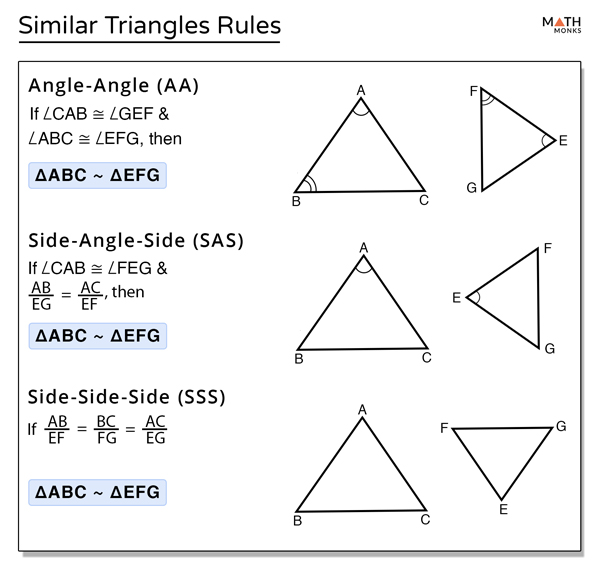
\includegraphics[scale=0.3]{imgs/Similar-Triangles-Rules.jpg}
                    \captionof{figure}{Similaridade de triângulos}
                \end{minipage}
                \begin{minipage}{.48\textwidth}
                \centering
                    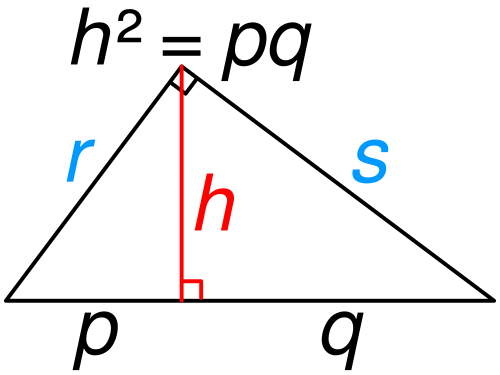
\includegraphics[scale=0.3]{imgs/Right_angle_altitude.png}
                    \captionof{figure}{Altura de triângulo retângulo}
                \end{minipage}
            \end{center}
            
            \paragraph{Trigonometria}
                \begin{center}
                    \begin{minipage}{.48\textwidth}
                        \centering
                        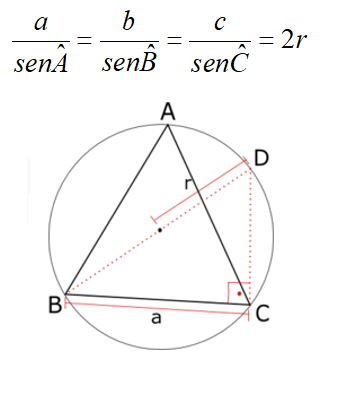
\includegraphics[scale=0.4]{imgs/leidossenos.png}
                        \captionof{figure}{Lei dos senos}
                    \end{minipage}
                    \begin{minipage}{.48\textwidth}
                    \centering
                        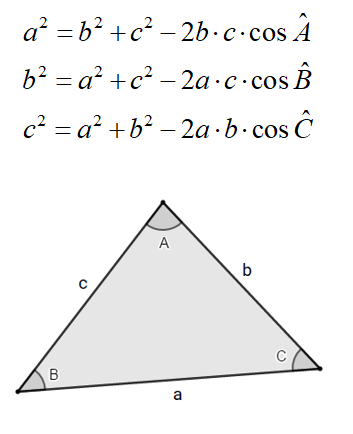
\includegraphics[scale=0.4]{imgs/leidoscosenos.png}
                        \captionof{figure}{Lei dos cossenos}
                    \end{minipage}
                    \begin{minipage}{.48\textwidth}
                    \centering
                        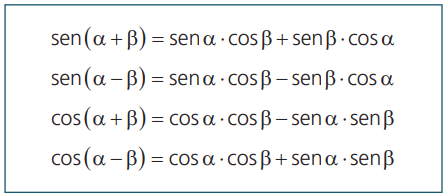
\includegraphics[scale=0.4]{imgs/soma_arcos.png}
                        \captionof{figure}{Soma de arcos}
                    \end{minipage}
                \end{center}
            
        \subsubsection{Fórmula de Heron}
        Calcular área de polígonos usando a medida dos lados, considere $a_i$ o $i$-ésimo lado e $p = \displaystyle \frac{\sum_{i=0}^n a_i}{2}$ o semiperímetro de um polígono.
            \begin{itemize}
                \item Triângulo: $A = \sqrt{p \cdot (p-a_0) \cdot (p-a_1) \cdot (p-a_2)}$
                \item Quadrilátero inscritível: $A = \sqrt{(p-a_0) \cdot (p-a_1) \cdot (p-a_2) \cdot (p-a_3)}$
                \item Quadrilátero qualquer: $A = \sqrt{(p-a_0) \cdot (p-a_1) \cdot (p-a_2) \cdot (p-a_3)  - a_0a_1a_2a_3 \cdot \cos(\frac{\alpha + \gamma}{2})}$, onde $\alpha,\gamma$ são ângulos opostos quaisquer
            \end{itemize}
    \subsection{Cálculo}
        \subsubsection{Multiplicadores de Lagrange}
        Dado uma função $f(x_1,x_2,\dots, x_n)$ com restrições $g_i(x_1,x_2,\dots,x_n) = k_i$ onde $1 \le i \le m$ e $m$ é o número de restrições, queremos otimizá-la. Usando o método dos multiplicadores de Lagrange, conseguimos reduzir o problema a resolver o sistema de equações:
        \[
            \left\{
            \begin{array}{{rcl}}
               \nabla f(x_1,x_2,\dots,x_n) & = & \sum_{i=1}^{m} \lambda_i \nabla g_i(x_1,x_2,\dots,x_n)  \\
                g_i(x_1,x_2,\dots,x_n)     & = & k_i \ \ \ \ \ \ \ \text{for $1 \le i \le m$}
            \end{array}
            \right.
        \]
        
        Para a primeira equação, você deriva a função para cada variável e resolve pra cada derivada parcial (vai ser um vetor de equações).

    \subsection{Polinômio}
        Se você acha que alguma função vira um polinômio de grau $k$, calcula o valor dessa função para $k+1$ valores e descobre os coeficientes do polinômio por um sistema linear. Exemplo $f(n) = \sum_{i=1}^n i$ pode ser um polinômio da forma $p(x) = ax^3 + bx^2 + cx + d$, calcula o valor de $f(n)$ para $0,1,2,3$ e calcula os coeficientes.
    \subsection{Teoria dos números}
        \subsubsection{Teorema de Fermat-Lagrange}
        \begin{minipage}{.48\textwidth}
        Todo inteiro pode ser escrito como:
        \begin{itemize}
            \item soma de no máximo 3 números triangulares,
            \item soma de no máximo 4 números quadrados,
            \item soma de no máximo 5 números pentagonais,
            \item \dots
        \end{itemize}
        O $i$-ésimo número $n$-gonal é a quantidade de pontos na construção do $i$-ésimo $n$-polígono conforme a figura. Sempre vai ter uma fórmula fechada para calcular esses números.
        \end{minipage}
        \begin{minipage}{.48\textwidth}
        \centering
        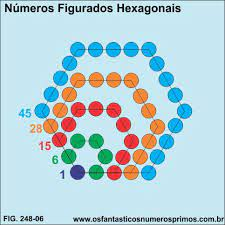
\includegraphics[scale=0.7]{imgs/ngonal.jpeg}
        \end{minipage}

        \subsubsection{Números primos}

        Todo $n \neq 2,3$ primo é da forma $6k \pm 1$. Pois qualquer outra forma de $6k + r$ com $0 \leq r < 5$ não é primo. Então você pode testar primo andando só de 6 em 6.
    \subsection{Probabilidade}
        \subsubsection{Valor esperado}
            Se $E(x) = \sum_{i=1}^x i\cdot P(x=i)$ com $P(x = i)$ sendo a probabilidade da variável $x$ ser igual a $i$, podemos reescrever como $E(x) = \sum_{i=1}^xP(x\geq i)$.
    \newpage

  
    
    \section{Inteiro Modular}
    Classe para lidar com problemas relacionados a operações modulares.
    
    \inputwithhash{./solutions/Math/modint.cpp}

      \section{Matrix Power}
    \subsection{Graph Paths I}
    You can use binary exponentiation to multiply the matrix to the $k$-eth exponent in $\mathcal{O}(\log_2(k))$. The complexity to multiply is $\mathcal{O}(N^3)$.
    
    Consider a directed graph that has $n$ nodes and $m$ edges. Your task is to count the number of paths from node $1$ to node $n$ with exactly $k$ edges.
    \inputwithhash{./solutions/Math/GraphPathsI.cpp}
    
    \subsection{Graph Paths II}
    Consider a directed weighted graph having $n$ nodes and $m$ edges. Your task is to calculate the minimum path length from node $1$ to node $n$ with exactly $k$ edges.
    \inputwithhash{./solutions/Math/GraphPathsII.cpp}

      \section{FFT}
    
    \subsection{Simple FFT}
    Multiplicação de dois polinômios em tempo $O((n+m) \cdot \log(n+m))$
    O polinômio $ a + bx + cx^2 + dx^3$ é representado na forma de vetor como $[a, b, c, d]$. Você passa dois $vector$ e a função $conv$ retorna os coeficientes do polinômio resultante.

    FFT é tudo sobre convolução, a multiplicação de dois polinômios é uma convolução. Convolução pode ser feita com funções contínuas ou discretas, a definição para funções contínuas seria:
    
    Dada duas funções contínuas por partes em $[0,\infty]$ a convolução de $f$ e $g$ é definida pela integral
        \[
            (f*g)(t) = \int_0^t f(r)g(t-r)dr
        \]

    Lib description: $fft(a)$ computes $\hat f(k) = \sum_x a[x] \exp(2\pi i \cdot k x / N)$ for all $k$ ($\exp(2\pi i \cdot kx/N) = e^{2\pi i \cdot kx/N} = w^i$, root of unity). $N$ must be a power of 2.
    Useful for convolution:
    \texttt{conv(a, b) = c}, where $c[x] = \sum a[i] \cdot b[x-i]$.
    For convolution of complex numbers or more than two vectors: FFT, multiply pointwise, divide by n, \texttt{reverse(start+1, end)}, FFT back. Rounding is safe if $(\sum a_i^2 + \sum b_i^2)\log_2{N} < 9\cdot10^{14}$
    (in practice $10^{16}$; higher for random inputs).
    Otherwise, use NTT/FFTMod. Time: $\mathcal{O}(N \log N)$ with $N = |A|+|B|$ ($\tilde 1s$ for $N=2^{22}$)
    \inputwithhash{./solutions/Math/fft.cpp}

    \subsection{FFT with random Mod}

     Lib description: Higher precision FFT, can be used for convolutions modulo arbitrary integers as long as $N\log_2(N)\cdot \text{mod} < 8.6 \cdot 10^{14}$ (in practice $10^{16}$ or higher). Inputs must be in $[0, \text{mod})$. Time: $\mathcal{O}(N \log N)$, where $N = |A|+|B|$ (twice as slow as NTT or FFT).

     \inputwithhash{./solutions/Math/fftmod.cpp}
     
    \subsection{FFT to solve String with Wildcards}
    Given two strings $s$ and $t$, with $t$ having wildcards that can match with any character, returns the number of ocurrence of $t$ in $s$.
    Solution $O(N\log_2(N))$.
    
    \bigskip
    
    (Original Problem: Maraton Nacional de Programacion Colombia 2016 - Wildcards).
    \inputwithhash{./solutions/Math/fft_wild_card.cpp}
    
    \subsection{FFT modular (NTT)}

    Lib description: $ntt(a)$ computes $\hat f(k) = \sum_x a[x] \cdot g^{xk}$ for all $k$, where $g=\text{root}^{(mod-1)/N}$. N must be a power of 2. Useful for convolution modulo specific nice primes of the form $2^a b+1$, where the convolution result has size at most $2^a$. For arbitrary modulo, see FFTMod. \texttt{conv(a, b) = c}, where $c[x] = \sum a[i] \cdot b[x-i]$. For manual convolution: NTT the inputs, multiply pointwise, divide by n, \texttt{reverse(start+1, end)}, NTT back. Inputs must be in $[0, \text{mod})$. Time: $\mathcal{O}(N \log N)$.
    
    To use a modular FFT, also known as NTT, you need a $n$-th root of ur modulus and then define some values in general u can say :
    
    $mod = x*2^k$
    
    $G = 3 $ or $5$
    
    $root = G^{mod/(2^k)}$
    
    $root_1 = root^{-1}$
    
    $root_{pw} = 2^k$
    \inputwithhash{./solutions/Math/ntt.cpp}

    \subsection{FWHT (fft using xor/and/or)}
    FFT but the expoent operation is xor/and/or.

    There are some crazy problems where u need to multiply $N$ polynomials of the form $x^0 + x^i$ and the $i$ can be up to $N$. the main approach is to use some D\&C to multiply those and to keep the polynomials divide in two parts. It is also coded down here. Operations can be modular.
    \inputwithhash{./solutions/Math/FWHT.cpp}

      \section{Gauss}

    \subsection{Simple Gauss}

    Used to solve system of linear algebraic equations (SLAE), determine if the SLAE has no solution, one or an infinite number of solutions. If we have a SLAE:
    
    \[
        \begin{matrix}
            a_{1,1}x_1 &+& a_{1,2}x_2 &+& \dots &+& a_{1,m}x_m &=& b_1 \\
            a_{1,1}x_1 &+& a_{1,2}x_2 &+& \dots &+& a_{1,m}x_m &=& b_2 \\
            \vdots     &+& \vdots     &+& \vdots&+& \vdots     &=& \vdots \\
            a_{n,1}x_1 &+& a_{n,2}x_2 &+& \dots &+& a_{n,m}x_m &=& b_n
        \end{matrix}
        \\  
    \]
    
    We can see it as matrices:
    
    \[
        A_{n,m} = \begin{bmatrix} 
            a_{1,1} & a_{1,2} & \dots & a_{1,m} \\
            a_{2,1} & a_{2,2} & \dots & a_{2,m} \\
            \vdots  & \vdots  &  \vdots& \vdots \\
            a_{n,1} & a_{n,2} & \dots & a_{n,m} 
        \end{bmatrix}
        \quad
        X_{m,1} = \begin{bmatrix} 
            x_{1,1} \\
            x_{2,1} \\
            \vdots  \\
            x_{m,1}  
        \end{bmatrix} 
        \quad
        B_{n,1} = \begin{bmatrix} 
            b_{1,1} \\
            b_{2,1} \\
            \vdots  \\
            b_{n,1}  
        \end{bmatrix} 
    \]

    Then the SLAE can be seen as $A_{n,m} \cdot X_{m,1} = B_{n,1}$, and we can solve it using Gauss-Jordan Elimination to remove linearly dependent equations (vectors) from the system. In the end, the number of non-zero equations is equal to the number of independent equations (vectors) of the system. We call this number the rank $r$ of the matrix, and $m-R$ is called the free parameter and refers to the number of free variables.

    Suppose we have an SLAE with rank $r$, let say that the free variables
    are $x_{m-r+1},x_{m-r+2},\dots,x_{m}$ and the other are $x_1,x_2,\dots,x_{m-r}$, every non-free variable is a linear combination of the free variables and a constant term.

    \[
    \begin{matrix}
        x_1 &=&  b'_1  &+& a'_{1,m-r+1}x_{m-r+1} &+& \dots &+& a'_{m}x_m \\
     \vdots &=& \vdots&+& \vdots &+& \vdots &+& \vdots \\
     x_{m-r}&=& b'_{m-r}&+& a'_{m-r,m-r+1}x_{m-r+1} &+& \dots &+& a'_mx_m \\
     x_{m-r+1} &=& s_{m-r+1} \\
     \vdots &=& \vdots \\
     x_m &=& s_m
    \end{matrix}
    \]

    $s_{m-r+1},\dots,s_m$ are any values from $\mathbb{R}$, we can write the set of solutions with vectors, and it forms a vectorial solution space.

    \[
        \begin{bmatrix}
            x_1 \\
            x_2 \\
            \vdots \\
            x_m
        \end{bmatrix}_{m,1}
         = \quad 
         \begin{bmatrix}
            b'_1 \\
            b'_2 \\
            \vdots \\
            b'_{m-r} \\
            0 \\
            0 \\
            \vdots \\
            0
        \end{bmatrix} _{m,1}
        + \quad
        s_{m-r+1}
        \begin{bmatrix}
            a'_{1,m-r+1} \\
            a'_{2,m-r+1} \\
            \vdots \\
            a'_{m-r,m-r+1} \\
            1 \\
            0 \\
            \vdots \\
            0
        \end{bmatrix}_{m,1}
        + \quad
        s_{m-r+2}
        \begin{bmatrix}
            a'_{1,m-r+2} \\
            a'_{2,m-r+2} \\
            \vdots \\
            a'_{m-r,m-r+2} \\
            0 \\
            1 \\
            \vdots \\
            0
        \end{bmatrix}_{m,1}
        + \dots + \quad
        s_{m}
        \begin{bmatrix}
            a'_{1,m} \\
            a'_{2,m} \\
            \vdots \\
            a'_{m-r,m} \\
            0 \\
            0 \\
            \vdots \\
            1
        \end{bmatrix}_{m,1}
    \]

    The first vector after the $=$ is one possible solutions, the other vectors compose a vectorial space of dimension $m-r$. This is the rank of the solution. We can say that $B_{n,1}$ is a linear combination of the columns of $A_{n,m}$.

    For each equation we search for a leading variable, a variable that isn't zero, after we find the "bigger one", we put it in the diagonal (change equations order and variables order). Then we update the values of the other coefficients (in the faster way, we don't need to update all the values of the matrix to make the column be zero). Then, we get the value for each variable.

    Lib description: Solves $A_{n,m} * X_{m,1} = B_{n,1}$, with $n$ being the number of equations and $m$ the number of variables. If there are multiple solutions, an arbitrary one is returned. Returns the solution alongside the vectors that generates all solutions. Time: $\mathcal{O}(n^2 m)$. The sizes of every vector must be correct.
    \inputwithhash{./solutions/Math/gauss.cpp}

    \subsection{Modular 2 (bitset)}
    Problem:
    
    a grid of switchs and each press in a switch i,j swaps the state of himself and the ones which are adjacent to it.
    
    If there is a way to make all on, print the switchs pressed.

    The $A$ matrix is equivalent to the augmented matrix $A|B$.
    \inputwithhash{./solutions/Math/gaussmod2.cpp}
    
    \subsection{Matrix rank}
    The rank of a matrix is the largest number of linearly independent rows/columns of the matrix. The rank is not only defined for square matrices.
    We can see that the other variables are "free", so can be uses to combinatorial problems.
    
    Example:
    
    Given a set of n integers, how many subsets have xor not equal to 0?
    \inputwithhash{./solutions/Math/subset-nim.cpp}

    \subsection{Xor Basis}

    Useful for bit problems of the type: "I have some numbers and I want to count how many distincts subset xor's exist". To do it we consider the vectorial space $\mathbb{Z}^d_2$ (vectors with $d$ positions and taken modulo 2). Each vector represents a number, the positions of the vector represents the bits of the number and the modulo 2 sum has the same behavior of xor operation, so we can treat the numbers as vectors of this space. Now the problem reduces to find how many vectors are linearly independent and the number of distincts xor's will be $2^{|B|}$ where $B$ is the set of independent vectors. We will store only the independent vectors, and there will be a maximum number of $d$ of them. For every vector $v$ that we try to insert in the basis, we iterate over the existing vectors of the base and use them to remove the bits of $v$. Each vector has an distinct higher/lower bit. Insert elements and check if an element can be made in $\mathcal{O}(d)$ such that $d$ is the number of bits.

    \inputwithhash{./solutions/Math/xorbasis.cpp}

      
    \section{Simplex}
    Maximize ${\textstyle \mathbf {c^{T}} \mathbf {x} }$
subject to ${\displaystyle A\mathbf {x} \leq \mathbf {b} }$ and ${\displaystyle \mathbf {x} \geq 0}$
    \inputwithhash{./solutions/Math/Simplex.cpp}

      
    \section{Implementation of Polynomials}
    Algorithm to find a root, and also to divide a poly by some (x+c).
    \inputwithhash{./solutions/Math/polynomials.cpp}

      
    \section{Combinatória}
    Soluções de combinatória.

    \inputwithhash{./solutions/Math/comb.cpp}

    \subsection{Princípio da Inclusão-Exclusão}
    %https://codeforces.com/blog/entry/64625
    Dado $n$ conjuntos $X_1,X_2,\dots,X_n$, queremos contar o tamanho da união deles, o seu tamanho é: 
    $$|X_1 \cup X_2 \cup \dots \cup X_n| = \sum_{k = 1}^{n} \left((-1)^{k-1} \cdot \sum_{s \in S_k} |s| \right)$$
    tal que que $S_k$ é o conjunto de todas as intersecções de $k$ conjuntos. De modo geral, podemos calcular isso em $\mathcal{O}(2^n)$ (iterar por todas as intersecções de conjuntos), mas podemos fazer em $\mathcal{O}(n)$ a depender da forma como calculamos $|s|$. Além disso, podemos fazer a mesma coisa para calcular a intersecção de conjuntos usando a união deles (onde é união vira intersecção, e onde é intersecção vira união).

    \subsubsection{Desarranjos}
    O número de desarranjos de $n$ números, expresso por $!n$, é igual ao número de permutações tal que nenhum elemento aparece em sua posição original, $p_i \neq i$ para $1 \le i \le n$. Para calcular isso, podemos pensar nos eventos $E_1,E_2,\dots,E_n$, tal que $E_i$ é a quantidade de permutações tal que na $i$-ésima posição, temos que $p_i = i$. Agora o problema virou calcular $n! - \sum_{i=1}^n E_i$, mas contar isso vai dar errado, pois estamos contando eventos repetidos em $\sum_{i=1}^n E_i$. Por exemplo, no cenário em que a posição $i$ e $j$ tem $p_i = i$ e $p_j = j$, vamos contar esse cenário em $E_i$ e $E_j$, ou seja, esses conjuntos tem intersecção não nula. Então o correto seria contar $n! - \left| \bigcup_{i=1}^n E_i \right|$, esse problema vira um problema de inclusão e exclusão (calcular a união de conjuntos). Uma intersecção de $k$ conjuntos vai ter tamanho igual a
    $$\binom{n}{k} \cdot (n-k)! = \frac{n!}{k!(n-k)!} \cdot (n-k)! = \frac{n!}{k!}$$ isso significa escolher $k$ elementos que vão estar fixos e outros elementos vão estar permutados de qualquer jeito. No fim, vamos calcular
    $$n! - \sum_{k=1}^n \left( (-1)^{k-1} \cdot \frac{n!}{k!}\right) = n! \sum_{k=1}^n \frac{(-1)^{k-1}}{k!}$$ que pode ser feito em $\mathcal{O}(n)$.

    \subsection{Números de Catalão}
    Sequência gerada pela recorrência $ C_n = \sum_{i=0}^{n-1}C_i \cdot C_{n-1-i}$, que tem fórmula fechada $C_n = \frac{1}{n+1} \binom{2n}{n}$.

    
    Para deduzir a fórmula fechada, primeiro pense em $C_n$ como a quantidade de expressões válidas com $2n$ parênteses. Disso podemos dizer que existem $\binom{2n}{n}$ maneiras de construir uma sequência de parênteses com $n$ parênteses abrindo e $n$ fechando (não necessariamente válidas). Disso vamos descontar as expressões inválidas. Considere que uma expressão inválida, ela vai conter um primeiro ponto no prefixo em que o número de parênteses fechando excede o número de parênteses abrindo por um, considere que vamos inverter todos os parênteses desse prefixo. Depois que invertemos vamos ter uma nova expressão com o total de $n+1$ parênteses abrindo e $n-1$ fechando, disso podemos dizer que toda expressão de parênteses inválida com $n$ abrindo e $n$ fechando pode ser mapeada para uma expressão de parênteses com $n+1$ abrindo e $n-1$ fechando (o método de inverter garante a bijeção dessa função). Então vamos ter $\binom{2n}{n+1}$ expressões inválidas. Assim, vamos ter $\frac{1}{n+1} \binom{2n}{n}$ expressões válidas.
    \[
       \binom{2n}{n} - \binom{2n}{n+1} = \binom{2n}{n} - \frac{n}{n+1} \cdot \binom{2n}{n} = \binom{2n}{n} \cdot \left( 1 - \frac{n}{n+1} \right) = \binom{2n}{n} \cdot \frac{1}{n+1}
    \]
    
    Alguns problemas clássicos envolvendo os números de catalão são:
    \begin{itemize}
        \item A quantidade de maneiras de criar uma expressão de $2n$ parênteses válida é igual a $C_n$.
        \item Quantidade de árvores binárias com $n$ nós é igual a $C_n$, a quantidade de árvores binárias enraizadas é igual a $C_{n-1}$.
    \end{itemize}

      
    \section{Lagrange Interpolation}
    Suppose you have a polynomial of order $N$, and want to find $f(X)$, and $X$ is really big. With Lagrange Interpolation, we can define any $f(x)$ as a linear combination of $N+1$ $f(u)$'s ($u$ is an arbitrary value, but we will use $1,2,\dots,k+1$). The normal approach is to calc the first $N+1$ answers and use them to calculate $f(X)$. Math below:

    Given the set of points $(x_0,f(x_1)),(x_2,f(x_2)),\dots,(x_k,f(x_N))$ that represent the polynomial $f(x)$ we can define auxiliary polynomials $f_i(x)$ such that (consider that $f(x_i) = y_i$):
    \[
    f_i(x) = \begin{cases}
    y_i, \text{ if } x = x_i \\
    0, \text{ if } x = x_j, j \neq i \\
    \text{some useless value otherwise}
    \end{cases}
    \] 
    This polynomial will look like $\displaystyle f_i(x) = y_i \cdot \prod_{j=0,j \neq i}^{N} \frac{x-x_j}{x_i-x_j}$, if we sum all the $f_i(x)$ polynomials we get an polynomial $g(x)$ such that $g(x_0) = y_0, g(x_1) = y_1, \dots, g(x_N) = y_N$, so $g = f$. Then $f(x) = \displaystyle \sum_{i=0}^N f_i(x) = \sum_{i=0}^N \left(y_i \cdot \prod_{j=0,j \neq i}^N \frac{x-x_j}{x_i-x_j}\right)$.

    The $y_i$ is an result of other function, so we pre-calculate that in $\mathcal{O}(N)$.

    \inputwithhash{./solutions/Math/lagrange.cpp}
    % Teoria dos numeros vai ter uma seção propria

      \section{Teoria dos Números}

    \subsection{Base e CRT}

    \inputwithhash{./solutions/Math/num_theory.cpp}

    \subsection{Diophantine}
    You have a equation $a \cdot x + b \cdot y = c$, you want to find values for $x$ and $y$ that satisfies it. The necessary and sufficient condition to the existence of a solution is that $c$ is a multiple of
$\gcd(a,b)$. Another situation is when you have $a \cdot x + b\cdot y = c \pmod{m}$, in this case, $c$ must be a multiple of $\gcd(a,b,m)$. 

    The problem narrows down to solving (where $g$ is the $\gcd$ of $a$ and $b$), so we can claim that, if there is a solution, there is a solution with $x < b$, similarly, there is a solution with $y < a$.
    \begin{cases}
        x \equiv (c/g)(a/g)^{-1}\pmod{b/g},\\
        y = \frac{c-ax}{b}.
    \end{cases}
    
    \subsection{Discrete Log}

    You have an modular equation with $a,b,x \in \mathbb{Z}$, you want to find a value for $x$ in $a^x \equiv b \;(\bmod\; m)$

    If you only want to find a solution, you just have to consider values between $[0,m-1]$ because, by the Pigeonhole Principle, $a^0,a^1,\dots,a^m$ you can only have m possible values, so minimally $a^m$ it's going to be a value that already appeared and it's going to cycle. So you have to consider values between $[0,m-1]$.

    However, the values of $m$ can be big, $10^9$, there's a way to solve it in $\sqrt{m}$ using the Baby-step Giant-step.

    Let's consider that $gcd(a,m) = 1$ and rewrite the expression (remember you can write every integer with $x = q*p + r$, where $0 \leq r < p$, and with that you can also write $x = (q+1)*p -r$, where $0 \leq r < p$):

    $$
    a^x \equiv b \mod{m} 
    $$
    $$
    a^{q*p-r} \equiv b \mod{m}
    $$
    $$
    a^{q*p}*a^{-r} \equiv b \mod{m}
    $$
    $$
    a^{q*p} \equiv b*a^r \mod{m}
    $$

    If you determine a good value for $p$, you can decrease the range of possible values of both $q$ and $r$, let $p = \sqrt{m}$, then $0 \leq p \leq \sqrt{m}+1$ (the plus 1 comes from the minus from the $r$) and $0 \leq r < \sqrt{m}$, so you can precalculate the values of $a^{q*p}$ for all $0 \leq p \leq \sqrt{m}$ and $b*a^{r}$ for all $0 \leq r < \sqrt{m}$, so in the end you have $O(\sqrt{m})$. And to find values of $q$ and $r$, you go through the values of $a^{q*p}$ and use binary search or two pointers to find which values $a^{q*p}$ and $b*a^r$ are equal.

    If $gcd(a,m) \neq 1$, then you can't calculate the inverse of $a^r$, however you can still try to solve it, let $g = gcd(a,m)$, if $g \nmid b$ then the equation doesn't have solution (if $g \mid a$ and $g \mid m$, then certainly, by linear combination, $g \mid b$). If $g \mid b$, then you can divide everyone by $g$. And do it until $gcd(a,m) \neq 1$. But after every time you do this operation you eliminate one $a$ from $a^x$.

    $$a^x \equiv b \mod{m}$$
    $$a^{x-1}*a \equiv b \mod{m}$$
    $$a^{x-1}*\frac{a}{g} \equiv \frac{b}{g} \mod{\frac{m}{g}}$$
    
    $$\dots$$
    
    $$a^{x-add}*\frac{a^{add}}{k} \equiv \frac{b}{k} \mod{\frac{m}{k}}$$

    After applying the operation $add$ times you have to solve the problem with new values where $gcd(a,\frac{m}{k}) \neq 1$. $\mathcal{O}(\sqrt{m})$ where $m$ is the mod.

    \inputwithhash{./solutions/Math/discrete_log.cpp}    

    \subsection{GCD Array Trick}
    Way to store all gcds in a array range . For each $i$ you store every different gcd sub-segment that exists starting at $i$.
    
    In this problem you need to find a $Max(gcd(A[l],\cdots,A[r])*(r-l+1))$. There is at most $\log_2(\max(A))$ distinct $\gcd$ values. 
    \inputwithhash{./solutions/Math/gcdrobado.cpp}
    
        

    \subsection{High Level Integer Fatorization}
    We can use this algorithms to find factors of greaters numbers.
    \subsubsection{Miller Rabin}

    Using the first 12 primes we can test if any number $\le 2^{64}$ is prime is $O(ln \textit{ n} )^2$
    
    \inputwithhash{./solutions/Math/miller.cpp}  

    The Polard Rho algoritms returns a non-trivial factor of a number. We can add this with the miller-Rabin to decompose the number testing this factor is a prime number.
    
    \subsubsection{Polard Rho}
    \inputwithhash{./solutions/Math/rho.cpp} 

    \subsection{Lucas Theorem}

    Given $n, k$ and $m$, find $\binom{n}{k}$ mod $m$, where $(n, k \le 10^{9})$, $m$ is a square-free number less than or equal to $10^{9}$ and each prime that appears on $m$ is less than $50$. A Square-Free number is a number that, in his prime factorization, each prime appears exactly once.

    \inputwithhash{./solutions/Math/Lucas.cpp}
    

    \subsection{Multiplicative Functions}
   In number theory, a multiplicative function is an arithmetic function $f(n)$ of a positive integer $n$ with the property that $f(1) = 1$ and

$$\displaystyle f(ab)=f(a)f(b)$$

whenever a and b are coprime.

    Examples of multiplicative functions:
    \begin{itemize}
        \item $gcd(n,k)$: the greatest common divisor of n and k, as a function of n, where k is a fixed integer.
\item {$\displaystyle \varphi (n)$}: Euler's totient function 
{$\displaystyle \varphi$ }, counting the positive integers coprime to (but not bigger than) $n$
\item $\mu (n)$: the Mobius function, the parity (-1 for odd, +1 for even) of the number of prime factors of square-free numbers; 0 if n is not square-free
\item $\sigma k(n)$: the divisor function, which is the sum of the k-th powers of all the positive divisors of n (where k may be any complex number). Special cases we have
\begin{itemize}
    \item $\sigma 0(n) = d(n)$ the number of positive divisors of n,
    \item $\sigma 1(n) = \sigma (n)$, the sum of all the positive divisors of n.
\end{itemize}
    \end{itemize}

    The main ideia of multiplicative functions is to use the linear sieve or just the sieve to calculate them. Normaly it will lead to some principle and u will need to calculate the solution to powers of primes and products of coprimes.
    for example we have for $\phi(x)$ that:
    \begin{itemize}
        \item $\phi(p) = p-1$,
        \item $\phi(p^k) = p^k -p^{k-1}$,
        \item $\phi(a*b) = \phi(a) * \phi(b)$, if $a$ and $b$ are coprime,
        \item $\phi(a*b) = \phi(a) * \phi(b) * \frac{gcd(a,b)}{\phi(gcd(a,b))}$, if $a$ and $b$ arent coprime,
    \end{itemize}

    Then we can calculate phi using sieve using the following code:

    \inputwithhash{./solutions/Math/phi.cpp}

    mantaining the quantity of the smallest prime can be useful to some functions, such as $f(p^k) = k$.

    \inputwithhash{./solutions/Math/fpk.cpp}
    \subsubsection{Mobius Inversion}

    The Mobius function which is in the list above have a really interesting property:

    lets define a function f as:

    $$
        f(x) = 
      \begin{cases}
        1, & \text{for } x = 1 \\
        0, & \text{otherwise.} 
      \end{cases}
    $$
    
    we have an interesting property which can be used to solve alot of multiplicative function related problems.

    $$
        f(x)  = \sum_{d|x}\mu(d)
    $$

    And $\mu(d)$ is calculated like:

    $$
        \mu(d) = 
    \begin{cases}
        1, & \text{for } d = 1 \\
        0, & \text{if n is not square free} \\
        (-1)^r & \text{for r distinct primes in d.}
    \end{cases}
    $$

    \inputwithhash{./solutions/Math/mobius.cpp}

    So lets say we need to calculate the following:
    \begin{align*}
        \sum_{i=1}^{n}& \sum_{j=1}^{n} [gcd(i,j) = 1] \\
        \sum_{i=1}^{n}& \sum_{j=1}^{n} \sum_{d|gcd(i,j)}\mu(d) \\
        \sum_{i=1}^{n}& \sum_{j=1}^{n} \sum_{d = 1}^{n} [d|gcd(i,j)]*\mu(d) \\
        \sum_{i=1}^{n}& \sum_{j=1}^{n} \sum_{d = 1}^{n} [d|i]*[d|j]*\mu(d) \\
       \sum_{d = 1}^{n}& \mu(d) * (\sum_{i=1}^{n}[d|i]) * (\sum_{j=1}^{n}[d|j]) \\
       \sum_{d = 1}^{n}& \mu(d) * (\left\lfloor \frac{n}{d} \right\rfloor) * (\left\lfloor \frac{n}{d} \right\rfloor) 
    \end{align*}

    So we started with a $O(N^2 * log(N))$ solution went to a $O(N^3 * log(N))$ solution, 
    but with the power of magic(known as math in some places) we ended with a $O(N)$ solution.

    Some other possible problems using this:
    
    \begin{align*}
        \sum_{i=1}^{n}& \sum_{j=1}^{n} gcd(i,j) \\
        \sum_{k=1}^{n}& \sum_{i=1}^{n} \sum_{j=1}^{n} [gcd(i,j) = k] \\
        \sum_{k=1}^{n}& k * \sum_{a=1}^{\left\lfloor \frac{n}{k} \right\rfloor} 
        \sum_{b=1}^{\left\lfloor \frac{n}{k} \right\rfloor} [gcd(a,b) = 1] \\
        \sum_{k=1}^{n}& k * \sum_{d = 1}^{\left\lfloor \frac{n}{k} \right\rfloor} \mu(d) * (\left\lfloor \frac{n}{d*k} \right\rfloor) * (\left\lfloor \frac{n}{d*k} \right\rfloor) 
    \end{align*}

    Next:

    \begin{align*}
        \sum_{i=1}^{n}& \sum_{j=1}^{n} lcm(i,j) \\
        \sum_{i=1}^{n}& \sum_{j=1}^{n} \frac{i*j}{gcd(i,j)} \\
        \sum_{k=1}^{n}& \sum_{i=1}^{n} \sum_{j=1}^{n} [gcd(i,j) = k]*\frac{i*j}{k} \\
        \sum_{k=1}^{n}& k * \sum_{a=1}^{\left\lfloor \frac{n}{k} \right\rfloor} 
        \sum_{b=1}^{\left\lfloor \frac{n}{k} \right\rfloor} [gcd(a,b) = 1]*a*b \\
        \sum_{k=1}^{n}& k * \sum_{d = 1}^{\left\lfloor \frac{n}{k} \right\rfloor} \mu(d) * (\sum_{a=1}^{\left\lfloor \frac{n}{k} \right\rfloor}[d|a]*a) * ( 
        \sum_{b=1}^{\left\lfloor \frac{n}{k} \right\rfloor} [d|b]*b) \\
        a =& d*p\text{, }b = d*q\\
        \sum_{k=1}^{n}& k * \sum_{d = 1}^{\left\lfloor \frac{n}{k} \right\rfloor} \mu(d) * (\sum_{p=1}^{\left\lfloor \frac{n}{k*d} \right\rfloor}d*p) * ( 
        \sum_{q=1}^{\left\lfloor \frac{n}{k*d} \right\rfloor} d*q) \\
       \sum_{k=1}^{n}& k * \sum_{d = 1}^{\left\lfloor \frac{n}{k} \right\rfloor} \mu(d) * d^2 * (\sum_{p=1}^{\left\lfloor \frac{n}{k*d} \right\rfloor}p) * ( 
        \sum_{q=1}^{\left\lfloor \frac{n}{k*d} \right\rfloor} q) \\
        \sum_{k=1}^{n}& k * \sum_{d = 1}^{\left\lfloor \frac{n}{k} \right\rfloor} \mu(d) * d^2 * (\sum_{p=1}^{\left\lfloor \frac{n}{k*d} \right\rfloor}p) * ( 
        \sum_{q=1}^{\left\lfloor \frac{n}{k*d} \right\rfloor} q) \\
        \text{the}&\text{ left part can be done with an PA, which will denoted as } PA(l,r)\\
        \sum_{k=1}^{n}& k * \sum_{d = 1}^{\left\lfloor \frac{n}{k} \right\rfloor} \mu(d) * d^2 * (PA(1,\left\lfloor \frac{n}{k*d} \right\rfloor)^2)  \\
        \text{let }& l = k*d\\
         \sum_{k=1}^{n}& k * \sum_{d = 1}^{\left\lfloor \frac{n}{k} \right\rfloor} \mu(d) * d^2 * (PA(1,\left\lfloor \frac{n}{l} \right\rfloor)^2)  \\
         \sum_{l=1}^{n}& (PA(1,\left\lfloor \frac{n}{l} \right\rfloor)^2) * \sum_{d'|l} \mu(d') * d' * l   \\
    \end{align*}

    Now lets analyze a problem with an vector $A$ with max element being $M$ and we need to calculate:


    \begin{align*}
        \sum_{i=1}^{n}& \sum_{j=1}^{n} lcm(A[i],A[j]) \\
        \sum_{d=1}^{M}& \sum_{(a \in A \And d|a)} \sum_{(b \in A \And d|b)} [gcd(\frac{a}{d},\frac{b}{d}) = 1] * \frac{a*b}{d} \\
        \sum_{d=1}^{M}& \sum_{(a \in A \And d|a)} \sum_{(b \in A \And d|b)} \sum_{l=1}^{M} \mu(l) * [l|\frac{a}{d}][l|\frac{b}{d}] * \frac{a*b}{d} \\
        \sum_{d=1}^{M}& \frac{1}{d} * \sum_{l=1}^{M} \mu(l) * ( \sum_{a \in A} \sum_{b \in A} [dl|a][dl|b] * a*b) \\
        \text{let }& t = dl\\
        \sum_{t=1}^{M}& \frac{1}{d} * \sum_{l|t} \frac{l}{t} * \mu(l) * ( \sum_{a \in A} \sum_{b \in A} [t|a][t|b] * a*b) \\
        \sum_{t=1}^{M}&(\sum_{l|t} \frac{l}{t} * \mu(l)) * ( \sum_{a \in A \And t|a} a)^2 
    \end{align*}

  

    
    \section{Nelsi's anotations}
    
        \subsection{Chicken McNugget Theorem}
            The Chicken McNugget Theorem (or Postage Stamp Problem or Frobenius Coin Problem) states that for any two relatively prime positive integers $m,n$, the greatest integer that cannot be written in the form $am + bn$ for nonnegative integers $a, b$ is $mn-m-n$.  
        
            A consequence of the theorem is that there are exactly $\frac{(m - 1)(n - 1)}{2}$ positive integers which cannot be expressed in the form $am + bn$.
        
        \subsection{Kaplansky's Lemma} 
            \subsubsection{Lemma 1}
                Given a set of size $N$, how many subsets of size $K$ that do not contain consecutive elements exist?
                
                Basically, we will rewrite the elements of our set as $+$ and $-$. Such that between each pair of $+$, there is a $-$. Initially, we will choose $K$ plus signs. Then, we will have $x_1$ minus signs before the first plus, $x_2$ between the first and the second, and so on, up to $x_{\scriptscriptstyle K+1}$.
                \begin{align*}
                    x_1, x_{\scriptscriptstyle K+1} &\ge 0\\
                    x_i > 0 \; \forall \; 2 &\le i \le K 
                \end{align*}
        
                We have $N-K$ minus signs to distribute. Since $x_2$ to $x_{\scriptscriptstyle K}$ are positive integers, we will express $x_1$ and $x_{\scriptscriptstyle K+1}$ as positive integers in the form of $x'_1-1$ and $x'_{\scriptscriptstyle K+1}-1$, resulting in the equation:
                
                
                $x'_1 - 1 + x_2 + x_3 + ... + x_{\scriptscriptstyle K-1} + x_{\scriptscriptstyle K} + x'_{\scriptscriptstyle K+1}-1 = N-K$
        
                $x'_1 + x_2 + x_3 + ... + x_{\scriptscriptstyle K-1} + x_{\scriptscriptstyle K} + x'_{\scriptscriptstyle K+1} = N - K + 2$
        
                
                We know the formula for calculating how many integer solutions there are for a positive integer.
        
                $\binom{M-1}{P}$ Assuming $M$ is the desired answer and $P$ is the number of coefficients.
        
                In our problem, it takes the following form: $\binom{N-K+1}{K}$
    
            \subsubsection{Lemma 2}
            Given a circle with numbers from $1$ to $N$, in how many ways can we choose $K$ numbers without selecting neighboring ones?

            We can divide the problem into $2$ cases:

            If N belongs to the set, we need to choose $K-1$ elements from $N-3$ options. Following the previous lemma, our answer is:
            
            $\binom{N-K-1}{K-1}$
            
            
            If N does not belong to the set, we have to choose $K$ from $N-1$ options.Following the previous lemma, our answer is:
            
            $\binom{N-K}{K}$

            
            Summing up the two answers we obtained, we have:  $\binom{N-K-1}{K-1}\binom{N-K}{K}$ $=$ $\frac{N}{N-K}\binom{N-K}{K}$
        \subsection{Divisor Analysis - CSES} 
            \subsubsection{Number of Divisors}
                    Each divisor of the number can be written as $\prod_{i = 1}^N x_i^{\alpha_i}$
                    where $0 \leq \alpha_i \leq k_i$.
                    
                    Since there are $k_i + 1$ choices for $\alpha_i$, the number of divisors is
                    simply $\prod_{i = 1}^N (k_i + 1)$.
                    
                    We can calculate this by iterating through the prime factors in $\mathcal O(N)$
                    time.
                    
            \subsubsection{Sum of divisors}
            
                Let the sum of divisors when only considering the first $i$ prime factors be $S_i$. The answer will be $S_N$.
                
                $$\begin{aligned} S_i &= S_{i - 1} \sum_{j = 0}^{k_i} x_i^j\\ &= S_{i - 1} \cdot \frac{x_i^{k_i + 1} - 1}{x_i - 1}\\ \end{aligned}$$
                
                We can calculate each $S_i$ using fast exponentiation and modular inverses in
            $\mathcal O(N \log(\max(k_i)))$ time.
            
            \subsubsection{Product of divisors}

                Let the product and number of divisors when only considering the first $i$ prime
                factors be $P_i$ and $C_i$ respectively. The answer will be $P_N$.
                
                $$\begin{aligned} P_i &= P_{i - 1}^{k_i + 1} \left(x_i^{k_i(k_i + 1)/2} \right)^{C_{i - 1}} \end{aligned}$$
                
                Again, we can calculate each $P_i$ using fast exponentiation in
                $\mathcal O(N \log(\max(k_i)))$ time, but there's a catch! It might be tempting
                to use $C_{i - 1}$ from your previously-calculated values in part 1 of this
                problem, but those values will yield wrong answers.
                
                This is because $a^b \not \equiv a^{b \bmod p} \pmod{p}$ in general. However, by
                Fermat's little theorem, $a^b \equiv a^{b \bmod (p - 1)} \pmod{p}$ for prime
                $p$, so we can just store $C_i$ modulo $10^9 + 6$ to calculate $P_i$.

        \subsection{Bracket Sequences II - CSES}
            For the "Bracket Sequences II" solution, we will first calculate the factorials and perform the following checks. Initially, we will check if the bracket sequence (BS) becomes irregular at any point; if it does, we return $0$. Additionally, we will verify if our right bracket sequence (RBS) has all $N$ elements; if it does, we return $1$.

            After these base case checks, we will proceed to calculate the Catalan number for this value.
 
            The standard formula for the Catalan number is:

            $C_n = \binom{2n}{n} - \binom{2n}{n - 1}$

            This formula means that out of the $2n$ opening parentheses, we will choose $n - 1$ to close. We will make a small modification to it. We will keep track of the number of parentheses that have already been opened and closed and substitute that into the formula. 

            $C_n = \frac{2n - (open + close)}{(n-open)!(n-close)!} - \frac{2n - (open + close)}{(n-open-1)!(n-close+1)!}$

  \section{Josephus Problem}

\subsection{Statement}

We are given the natural numbers $n$ and $k$.
All natural numbers from $1$ to $n$ are written in a circle. 
First, count the $k$-th number starting from the first one and delete it.
Then $k$ numbers are counted starting from the next one and the $k$-th one is removed again, and so on.
The process stops when one number remains.
It is required to find the last number.

This task was set by \textbf{Flavius Josephus} in the 1st century (though in a somewhat narrower formulation: for $k = 2$).

This problem can be solved by modeling the procedure.
Brute force modeling will work $O(n^{2})$. Using a Segment Tree, we can improve it to $O(n \log n)$.
We want something better though.

\subsection{Modeling a $O(n)$ solution}

We will try to find a pattern expressing the answer for the problem $J_{n, k}$ through the solution of the previous problems.

Using brute force modeling we can construct a table of values, for example, the following:

$$\begin{array}{ccccccccccc}
n\setminus k & 1 & 2 & 3 & 4 & 5 & 6 & 7 & 8 & 9 & 10 \\
1 & 1 & 1 & 1 & 1 & 1 & 1 & 1 & 1 & 1 & 1 \\
2 & 2 & 1 & 2 & 1 & 2 & 1 & 2 & 1 & 2 & 1 \\
3 & 3 & 3 & 2 & 2 & 1 & 1 & 3 & 3 & 2 & 2 \\
4 & 4 & 1 & 1 & 2 & 2 & 3 & 2 & 3 & 3 & 4 \\
5 & 5 & 3 & 4 & 1 & 2 & 4 & 4 & 1 & 2 & 4 \\
6 & 6 & 5 & 1 & 5 & 1 & 4 & 5 & 3 & 5 & 2 \\
7 & 7 & 7 & 4 & 2 & 6 & 3 & 5 & 4 & 7 & 5 \\
8 & 8 & 1 & 7 & 6 & 3 & 1 & 4 & 4 & 8 & 7 \\
9 & 9 & 3 & 1 & 1 & 8 & 7 & 2 & 3 & 8 & 8 \\
10 & 10 & 5 & 4 & 5 & 3 & 3 & 9 & 1 & 7 & 8 \\
\end{array}$$

And here we can clearly see the following \textbf{pattern}:

$$J_{n,k} = \left( (J_{n-1,k} + k - 1) \bmod n \right) + 1$$

$$J_{1,k} = 1$$

Here, 1-indexing makes for a somewhat messy formula; if you instead number the positions from 0, you get a very elegant formula:

$$J_{n,k} = (J_{n-1,k} + k) \bmod n$$

So, we found a solution to the problem of Josephus, working in $O(n)$ operations.

\subsection{Implementation}

Simple \textbf{recursive implementation} (in 1-indexing)

\begin{verbatim}
int josephus(int n, int k) {
    return n > 1 ? (josephus(n-1, k) + k - 1) % n + 1 : 1;
}
\end{verbatim}

\textbf{Non-recursive form}:

\begin{verbatim}
int josephus(int n, int k) {
    int res = 0;
    for (int i = 1; i <= n; ++i)
  	  res = (res + k) % i;
    return res + 1;
}
\end{verbatim}

This formula can also be found analytically.
Again here we assume 0-indexing.
After we delete the first number, we have $n-1$ numbers left.
When we repeat the procedure, we will start with the number that had originally the index $k \bmod n$.
$J_{n-1, k}$ would be the answer for the remaining circle, if we start counting at $0$, but because we actually start with $k$ we have $J_{n, k} = (J_{n-1,k} + k) \ \bmod n$.

\subsection{Modeling a $O(k \log n)$ solution}

For relatively small $k$ we can come up with a better solution than the above recursive solution in $O(n)$.
If $k$ is a lot smaller than $n$, then we can delete multiple numbers ($\lfloor \frac{n}{k} \rfloor$) in one run without looping over.
Afterwards we have $n - \lfloor \frac{n}{k} \rfloor$ numbers left, and we start with the $(\lfloor \frac{n}{k} \rfloor \cdot k)$-th number.
So we have to shift by that many.
We can notice that $\lfloor \frac{n}{k} \rfloor \cdot k$ is simply $-n \bmod k$.
And because we removed every $k$-th number, we have to add the number of numbers that we removed before the result index.
Which we can compute by dividing the result index by $k - 1$.

Also, we need to handle the case when $n$ becomes less than $k$. In this case, the above optimization would cause an infinite loop.

\textbf{Implementation} (for convenience in 0-indexing):

\begin{verbatim}
int josephus(int n, int k) {
    if (n == 1)
        return 0;
    if (k == 1)
        return n-1;
    if (k > n)
        return (josephus(n-1, k) + k) % n;
    int cnt = n / k;
    int res = josephus(n - cnt, k);
    res -= n % k;
    if (res < 0)
        res += n;
    else
        res += res / (k - 1);
    return res;
}
\end{verbatim}

Let us estimate the \textbf{complexity} of this algorithm. Immediately note that the case $n < k$ is analyzed by the old solution, which will work in this case for $O(k)$. Now consider the algorithm itself. In fact, after every iteration, instead of $n$ numbers, we are left with $n \left( 1 - \frac{1}{k} \right)$ numbers, so the total number of iterations $x$ of the algorithm can be found roughly from the following equation:

$$ n \left(1 - \frac{1}{k} \right) ^ x = 1, $$

on taking logarithm on both sides, we obtain:

$$\ln n + x \ln \left(1 - \frac{1}{k} \right) = 0,$$ 
$$x = - \frac{\ln n}{\ln \left(1 - \frac{1}{k} \right)},$$

using the decomposition of the logarithm into Taylor series, we obtain an approximate estimate:

$$x \approx k \ln n$$

Thus, the complexity of the algorithm is actually $O (k \log n)$.

\subsection{Analytical solution for $k = 2$}

In this particular case (in which this task was set by Josephus Flavius) the problem is solved much easier.

In the case of even $n$ we get that all even numbers will be crossed out, and then there will be a problem remaining for $\frac{n}{2}$, then the answer for $n$ will be obtained from the answer for $\frac{n}{2}$ by multiplying by two and subtracting one (by shifting positions):

$$ J_{2n, 2} = 2 J_{n, 2} - 1 $$

Similarly, in the case of an odd $n$, all even numbers will be crossed out, then the first number, and the problem for $\frac{n-1}{2}$ will remain, and taking into account the shift of positions, we obtain the second formula:

$$J_{2n+1,2} = 2 J_{n, 2} + 1 $$

We can use this recurrent dependency directly in our implementation. This pattern can be translated into another form: $J_{n, 2}$ represents a sequence of all odd numbers, "restarting" from one whenever $n$ turns out to be a power of two. This can be written as a single formula:

$$J_{n, 2} = 1 + 2 \left(n-2^{\lfloor \log_2 n \rfloor} \right)$$

\subsection{Analytical solution for $k > 2$}

Despite the simple form of the problem and a large number of articles on this and related problems, a simple analytical representation of the solution of Josephus' problem has not yet been found. For small $k$, some formulas are derived, but apparently they are all difficult to apply in practice (for example, see Halbeisen, Hungerbuhler "The Josephus Problem" and Odlyzko, Wilf "Functional iteration and the Josephus problem").

\chapter{Data Structures}
  \section{Dicas}
\begin{itemize}
    \item BINARY JUMPING EXISTE.
    \item Quer update em $\mathcal{O}(1)$? SQRT Decomposition neles.
    \item Update em range? No vetor de diferença talvez altere só duas posições (o prefixo do vetor de diferença é a mudança real na posição).
\end{itemize}

  \section{Ordered Set}
Same as Set, but with two new queries
\begin{itemize}
    \item s.order\_of\_key$(k)$: Number of items strictly smaller than $k$ .
    \item s.find\_by\_order$(k)$: $k$-th element in a set (counting from zero).
\end{itemize}

\inputwithhash{./solutions/DataStructures/oset.cpp}
  \section{Fenwick Tree}
\subsection{2D}

You are given an n×n grid representing the map of a forest. Each square is either empty or has a tree. Your task is to process q queries of the following types:
Change the state (empty/tree) of a square.
How many trees are inside a rectangle in the forest? You can use the magic of Inclusion and Exclusion to solve this one. $\mathcal{O}(\log^2(N))$ per update and query.

\inputwithhash{./solutions/DataStructures/ForestQueriesII.cpp}

\subsection{Fenwick Lifting}
Binary search on a BIT in $O(log(N))$

\inputwithhash{./solutions/DataStructures/fenwick_lifting.cpp}

  \section{Sparse Table}

\subsection{Simple Sparse table}
Idempotent queries in $O(1)$, others $O(\log (n))$.
\inputwithhash{./solutions/DataStructures/sparsetable.cpp}
\subsection{Disjoint Sparse table}
All kind of queries in $O(1)$.
\inputwithhash{./solutions/DataStructures/sparsetabledisjoint.cpp}
  \section{SQRT Decomposition}

\subsection{MO}

In the Persistent DSU section, there is a very hard application of MO. Solve static queries in offline in $\mathcal{O}(Q\cdot \sqrt{N})$ where $Q$ is the number of queries and $N$ the vector size.
\inputwithhash{./solutions/DataStructures/mo.cpp}

\subsection{MO com queries}

Um ponto importante é que se nós fizermos aquele esquema de decompor a query de path em arvore em uma query no range do euler tour, também podemos usar mo. 
\inputwithhash{./solutions/DataStructures/moupdate.cpp}

\subsection{Blocking}
We partition the array into blocks of size $\texttt{block\_size}=\lceil \sqrt{N} \rceil$. Each block stores the answer for the elements within it.

Update in $\mathcal{O}(1)$. To update an element at location $x$, find the block of it ($\frac{x}{\texttt{block\_size}}$), remove the $x$ contribution and add the new one.

Query in $\mathcal{O}(\sqrt{N})$. For each complete block between the $(l,r)$ of the query, add the already calculated contribution, for the left and right part iterate over it.
Since there is at most $\sqrt{N}$ blocks and each block has $\sqrt{N}$ of size, we at most iterate $\sqrt{N}*3$.
\inputwithhash{./solutions/DataStructures/blocking.cpp}

\subsection{Blocking com cyclic shift}
Legendary Huron is a fan of beautiful fences. He defines the beauty of a sequence (l,r) is $max_{l \leq i \leq j \leq r}(a[j]-a[i])$
Queries

Given three integers l, r, k, he will repaint the planks in the range [l,r]. With a[l] = k, a[l+1] = k+1 ...;
Given two integers l and r, returns the beauty.
\inputwithhash{./solutions/DataStructures/sqrtdecomp.cpp}

\subsection{Batching}
Maintain a "buffer" of the latest updates (up to $\sqrt N$). The answer for each
sum query can be calculated with prefix sums and by examining each update within
the buffer. When the buffer gets too large ($\ge \sqrt N$), clear it and
recalculate prefix sums.

\inputwithhash{./solutions/DataStructures/batching.cpp}

          
    \section{Implicit Treap}
    Basicamente é uma estrutura que dá pra fazer um monte de coisa com "pouco"  código. A operação reverse é a + roubada. A complexidade é $\mathcal{O}(N\log^2(N))$, mas chutando alto, às vezes dependendo pode ser mais rápido.
    
    % \lstinputlisting{./solutions/DataStructures/Treap.cpp}

    Wevton version. %Essencialmente é a mesma usada acima, mas coloquei dentro de uma struct e fiz mais algumas funções que parecem ser comuns em problemas envolvendo Treaps. Por algum motivo que eu não sei, ela é alguns milisegundos mais rápida que a Treap acima.
    
    \inputwithhash{./solutions/DataStructures/Treap_Wevton.cpp}

  \section{DSU}
Diferentes implementações com diferentes focos.

\subsection{DSU com Small to Large}
Quando além do DSU, você tem outras informações sobre os grupos que vão ser alteradas quando você realizar a união dos grupos. $\mathcal{O}(N\log(N)\cdot T)$ tal que $T$ é o custo de realizar a união (relacionado com as informações de cada grupo).
\inputwithhash{./solutions/DataStructures/DSU_SMOL.cpp}

\subsection{Persistent DSU}
Just a DSU such that you can ask who was my parent in time $t$.
\inputwithhash{./solutions/DataStructures/dsu_rollback_1.cpp}


\subsection{DSU with rollback}
A DSU such that you can roll back last operation.
\inputwithhash{./solutions/DataStructures/dsu_rollback_2.cpp}


\subsection{Connected Components With Segments}

Here start the crazy applications.

First one, given some set of edges, answer multiples queries. For each query answer how many connected components are there, if u use the edges in range (l,r).

The solution does an approach with mo and dsu with rollback. The main ideia is:

First solve for those such that $(r-l+1) < \sqrt(N)$. Just brute with DSU.
After it, lets split the solution in blocks of $l$. 
For each block u sort the queries by r. Lets say u are in first block and every $l$ lies in range $1--\sqrt{N}$.
The solution does the following steps:
\begin{itemize}
    \item Add every edge in range $\sqrt{N}+1-r$.
    \item Add every edge in range $l-\sqrt{N}$.
    \item get answer for this segment.
    \item rollback the edges in range $l-\sqrt{N}$.
    \item go to the next segment.
\end{itemize}

The first step can be slow, but for each block the amortized time will be $N$. The other steps, take $\sqrt{N}$ time.

\inputwithhash{./solutions/DataStructures/ConnectedComponentsWithSegments.cpp}

\subsection{Dynamic Connectivity Offline}

Solve those queries:
\begin{itemize}
    \item add an edge $u - v$
    \item remove an edge $u - v$
    \item answer the number off connected components.
\end{itemize}

The main idea is to define an id to each query of type $3$ and define ranges off "activation" suppose u add an edge $u - v$ and after it u remove. This will create a range $l - r$ which represents which queries off type $3$ this edge is active.

After it we will do a "segment tree" alike solution.

The main idea is to keep the segments which are relevant to this part of the queries and just add the edge when it cover all the ids in this segment. after it u always roll back the edges added in this level. it is easy to see (maybe it is not) that each segment will have a complexity close to a query in a segment tree.

\inputwithhash{./solutions/DataStructures/DynamicConnectivityOffline.cpp}

  \section{Linked List}

We can use this structure to add/erase elements in any position of an array. In normal case the cost of a linked list is $\mathcal{O}(n)$ but we can use a map to do the query of iterator in log. In this problem we need to add $i$ after a number $j$. And erase all elements between $a$ and $b$.

\inputwithhash{./solutions/DataStructures/linked_list.cpp}

  \section{Monotonic Stack}

You want to make queries of a lot of contiguous subsegments in a sliding window way, you can use Monotonic Stacks. The ideia is to mantain 2 queues, one queue represents a preffix of a subsegment and the other a suffix, the first element of the preffix stores the operation on the preffix and the last element of the suffix stores the operation on the suffix. Insert, remove and query in $\mathcal{O}(1)$.

\inputwithhash{./solutions/DataStructures/MonSt.cpp}

  \section{Range Minimum Queries}

Fazer pergunta de mínimo em um vetor em $\mathcal{O}(1)$. Brunomont neles.

\inputwithhash{./solutions/DataStructures/rmq.cpp}
  \section{Interval Manager}
Estrutura de dados para lidar com união de intervalos em $\mathcal{O}(\log(N))$ por inserção.

\inputwithhash{./solutions/DataStructures/IntervalManager.cpp}
  \section{Persistent Data Structures}
Some implementations of some persistent data Structures.

\subsection{Persistent Array}
\inputwithhash{./solutions/DataStructures/PersArray.cpp}

\subsection{Persistent Stack}
\inputwithhash{./solutions/DataStructures/PersStack.cpp}
  \section{Estruturas de Dados para Múltiplas Dimensões}
Códigos para fazer queries em múltiplas dimensões, só roubei do arthur9548 XD.

\subsection{Soma de Prefixos}
\inputwithhash{./solutions/DataStructures/psumMD.cpp}

\subsection{Fenwick Tree}
\inputwithhash{./solutions/DataStructures/fenwickMD.cpp}

\subsection{Segment Tree}
\inputwithhash{./solutions/DataStructures/segtreeMD.cpp}

\subsection{Sparse Table}
\inputwithhash{./solutions/DataStructures/sparsetableMD.cpp}

\subsection{Disjoint Sparse Table}
\inputwithhash{./solutions/DataStructures/distMD.cpp}
\chapter{Segment Tree}
  \section{Sem Lazy}
Seg Iterativa, é mais rápida
\inputwithhash{./solutions/DataStructures/Segtree/segtree.cpp}

  \section{Com Lazy}
Lazy updates must distribute over operations. $ch(op(a,b),x) = op(ch(a,x),ch(b,x))$ and $ch(a,cmp(x,y)) = ch(ch(a,x),y)$.
\inputwithhash{./solutions/DataStructures/Segtree/segtreelazy.cpp}
  \section{Implícita/Esparsa com Lazy}
\inputwithhash{./solutions/DataStructures/Segtree/implicityseg.cpp}
  \section{Persistente}

\inputwithhash{./solutions/DataStructures/Segtree/persistent_segtree.cpp}

Solution for Spoj Count on a Tree,
Given a tree there are $Q$ queries where you need to find the $k$th minimum weigth in a path between $u$ and $v$, it also needs the lca and lca's father between $u$ and $v$.

You make a Segtree for each path from the root to each node. And walk on the Seg to get the sum from the path of the root to the queries minus the sum of the root to LCA.

Queries in $O(log(n))$

\inputwithhash{./solutions/DataStructures/Segtree/CountOnATree.cpp}

\subsection{Persistente com Lazy}

\inputwithhash{./solutions/DataStructures/Segtree/persistent_lazy.cpp}

  \section{Contar minimos (união de area de retangulos)}

We would like a data structure that can efficiently handle two types of operations: Update index $i$ to value $v$ and report the minimum and the number of occurences of the minimum on a range $[l, r]$.

We can use a normal segment tree to handle range queries, but slightly modify each node and the merge operation. Let each node be a pair of values $(\texttt{val}, \texttt{cnt})$, where $\texttt{val}$ is the minimum value and $\texttt{cnt}$ is the number occurences of the minimum value.

If node $c$ has two children $a$ and $b$, then if $a.\texttt{val} < b.\texttt{val}$, then $c = a$.
If $a.\texttt{val} > b.\texttt{val}$, then $c = b$.
If $a.\texttt{val} = b.\texttt{val}$, then $c = \{a.\texttt{val}, a.\texttt{cnt} + b.\texttt{cnt}\}$. O problema clássico é unir a área de vários retângulos, o código faz isso.

\inputwithhash{./solutions/DataStructures/Segtree/AreaofRectangles.cpp}
  
    \section{Merge Sort Tree}

    Very strong Data Structure to answer queries but you can't do updates. A problem of this kind is something like that "You have an array and want to answer some queries on it, these queries are: given $l,r,x$ with $l \le x \le r$, how many elements in this range are greater than $x$?"

    The idea is that each node of your tree is an array of elements now, and you will maintain a sorted array in each node. To answer the query, one must do a binary search in each node of the range to find how many of the elements are greater than $x$. Time complexity of this is $\mathcal{O}(n\log^2(n))$. The same as a Seg, but just use \texttt{std merge} function, it goes like \texttt{merge(v1.begin(),v1.end(),v2.begin(),v2.end(),v.begin())}, where you will merge \texttt{v1 and v2} into \texttt{v}.
    \inputwithhash{./solutions/DataStructures/Segtree/MergeSortTree.cpp}

      
    \section{Segment Tree Beats}
    Updates:
    \begin{itemize}
        \item min(a[i],x) - range l - r
        \item max(a[i],x) - range l - r
        \item a[i]+=x - range l - r
    \end{itemize}
    Query:
    \begin{itemize}
        \item sum ai - range l-r
    \end{itemize}

    The complexity is $O(N\log^2(N))$.
    \inputwithhash{./solutions/DataStructures/Segtree/segbeats.cpp}

      \section{Wavelet Tree}
    Encontra o kth menor valor num range [L,R] com queries em $\mathcal{O}(\log(n))$. Espaço e pré-processamento é em $\mathcal{O}(n \log(n))$. Isso é do Kataki e tecnicamente é uma seg tree. \textbf{p} é o L e \textbf{q} é o R na query, o resto aceita que funciona.
    \inputwithhash{./solutions/DataStructures/Segtree/wavelet_tree.cpp}

\chapter{Dynammic Programming}
  \section{Dicas}
\begin{itemize}
    \item Mudar a ordem que você calcula a DP pode te otimizar um estado e pode facilitar a implementação;
    \item Você não precisa sempre calcular a DP numa ordem bonitinha (de $1$ até $N$), você pode ordenar os elementos e fazer a DP nessa nova ordem, pegada divisão e conquista e etc;
    \item Às vezes, nem todos os estados da DP são úteis (precisam ser visitados) e, às vezes, você só vai ``usar'' um estado um número limitado de vezes.
    \item Cuidado como você faz as transições. Se você tem uma DP que é do tipo $dp(i) = \sum_{k \in S}dp(k)$, tal que $S$ é um conjunto com valores sem padrão. Ao invés de para cada $dp(i)$ olhar para todos os $k$'s, pode ser melhor para cada  $k$ colocar a contribuição dele em $i$.
    \item Problema que é do tipo, você tem $N$ items, você pode fazer $M$ operações, na $i$-ésima operação, você perde $A_i$ itens e ganha $B_i$ pontos, qual o máximo de pontos que você pode ganhar? Pra resolver isso você vai usar o melhor item muitas vezes até você chegar numa pontuação $N' \leq LIM$ tal que $LIM$ vai normalmente ser alguma coisa na ordem de vai normalmente ser alguma coisa na ordem de $(\max(A_i))^2$, porque a ideia é que, sabendo do melhor item, você pode usar outros itens para mudar sua pontuação resto $\max(A_i)$ e nó máximo você vai realizar operações com itens piores $\max(A_i)$ vezes (mudar o módulo de 1 em 1).
\end{itemize}
  \section{Exchange Arguments}

\subsection{Dicas}
\begin{itemize}
    \item Talvez a função piso não faça diferença no Exchange Arguments (faz as contas pra ver).
\end{itemize}

You use the exchange arguments to proof that there is an ideal order of the elements. It's easy to see 
by an example problem.

Example: There are $N$ blocks, numbered $1,2,\dots, N$. For each $i$ ($1 \le i \le N$), 
block $i$ has a weight of $w_i$, a solidness of $s_i$ and a value of $v_i$. Taro has decided to build 
a tower by choosing some of the $N$ blocks and stacking them vertically in some order. Here, the tower 
must satisfy the following condition: for each block $i$ in the tower, the sum of the weights of the 
blocks stacked above it's not greater than $s_i$. Find the maximum possible sum of the values of the 
block contained in the tower.

Think about how you would order the blocks if there were only 2 of them, let's say the first has $w_1$ 
and $s_1$ and the second has $w_2$ and $s_2$. Let's consider both orderings and see what is the best 
one:
\begin{itemize}
    \item If you put the first on the bottom, the strength of the tower will be $s_1-w_2$.
    \item If you put the second on the bottom, the strength of the tower will be $s_2-w_1$.
\end{itemize}

So we want to take the first as the bottom one if $s1-w2 > s2-w1$. Which is equal to saying $s1+w1 > s2+w2$. Then, we want to put the ones with greater $s+w$ on the bottom. We have an ideal ordering of the elements, we make a dp using this order.
\inputwithhash{./solutions/DP/Tower.cpp}

  \section{Exponenciação de Matriz}

Quando a DP é uma recorrência linear, podemos representar a transição da DP como uma multiplicação 
de matrizes e utilizar a exponenciação de matrizes para calcular estados muito grandes da DP em 
$\mathcal{O}(\log(n) * M^3)$, tal que $M$ é a dimensão da matriz.
  \section{Fast Knapsack 3k trick}
Suponha que você tem um conjunto $A$ com $N$ valores e $\sum_{i=0}^{N-1} a[i] = M$.
Queremos calcular quais possiveis somas podemos obter. 

Primeiro, se todos os valores são distintos $ N < \sqrt{M}$. Se não, podemos representar os $K$ 
caras iguais a $x$ como sendo $x, 2x, 4x, \dots$ até o maior $2^i < K$ assim esses elementos 
representaram a mesma soma que os anteriores (você possivelmente vai guardar mais de um cara do 
tipo $x$ por exemplo, mas o ponto eh que a mochila de quais somas você consegue formar não vai ser 
alterada com essa transformação). Chegando numa solução que tem complexidade $O(M*\sqrt M)$. se for 
só um subset sum, podemos ainda usar um bitset.

Exemplo: You are in a book shop which sells $n$ different books. You know the price $h[i]$, the number 
of pages $s[i]$ and the number of copies of each book $k[i]$. You have decided that the total price of 
your purchases will be at most $x$. What is the maximum number of pages you can buy? You can buy 
several copies of the same book.

\inputwithhash{./solutions/DP/BookShopII.cpp}
  \section{SOS DP}
Sum over subsets (SOS) DP is a trick that allows you to efficiently compute the sum of all the subsets of an array.

The naive solution would be to iterate through every pair of masks and check if one of them is a subset of the other. We can speed this up if we iterate over only subsets of the current mask and add up all of the those values to get the sum over subsets for a particular mask ($\mathcal{O}(3^n)$).

The difference comes from the fact that in the first example we iterate over every pair of subsets which takes $(2^n)^2$ time and the second we iterate directly over the subsets for each mask. This means each mask is only visited by $2^{n - k}$ other masks where k is the number of elements of the mask.

This means that the total time complexity is O($\sum_{0}^{n} {n \choose k} \cdot 2^{n - k} = 3^n$).

Notice how in both of these examples we don't seem to be saving much information between different subsets which is the essence of DP.
Define $\texttt{SOS}(\texttt{mask}, x)$ to be the sum of subsets of mask such that the first $x$ bits of the subset are identical to the first $x$ bits of mask.
For example, $\texttt{SOS}(1001001, 3)$ includes the subsets $1001001$, $1000001$, $1001000$, $1000000$ which all have the same common prefix of $100$.

\[
\texttt{SOS}(mask, x) = \begin{cases}
    \texttt{SOS}(\texttt{mask}, x - 1) + \texttt{SOS}(\texttt{mask} - 2^i, x - 1)  \quad \textrm{if } |2^i \wedge \texttt{mask}| > 0 \\

    \texttt{SOS}(\texttt{mask}, x - 1) \quad \textrm{otherwise}  
\end{cases}
\]


One example is: given a list of $n$ integers, your task is to calculate for each element $x$:

\begin{itemize}
    \item The number of elements $y$ such that $x~|~y=x$, can be seen as $y \subseteq x$.
    \item the number of elements $y$ such that $x~\&~y=x$, that is equal to $(!x)~|~(!y)=~!x$, can be seen as $(!y) \subseteq (!x)$.
    \item the number of elements $y$ such that $x~\&~y\neq0$, that is the complement of to $(!x)~|~y=~(!x)$, can be seen as $y \subseteq (!x)$.
\end{itemize}

The solution of the problem is in $\mathcal{O}(X\cdot \log(X))$, where $X$ is the greatest element.

\inputwithhash{./solutions/DP/BitProblem.cpp}
  \section{Permutation Tricks}

\subsection{Trick 1}

The main ideia is that $dp(N)$ stores a permutation of $N$ elements, when considering $dp(N+1)$ we 
think of it as putting a new element with value equal to $X$ in the end, then all the elements greater 
than or equal to $X$ will be $+1$, the ones that are lower don't change. This guarantee that the final 
vector is also a permutation independently of the value of $X$.

Example: Your task is to count the number of permutations of $1,2, \ldots ,n$ that have exactly $k$ inversions. Consider $dp(i,j) =$ permutations with $i$ elements and $j$ inversions. Then $dp(i,j) =  \sum_{x = 1}^{i} dp(i-1,j-(i-k))$. In this problem you need to do some optmizations with preffix sum.
\inputwithhash{./solutions/DP/PermutationInversions.cpp}

\subsection{Trick 2}

The main idea is to think to build the permutation starting from an empty vector, the process of building consists in putting the elements in an order. In some step of the process you will have a permutation of $N$ element, the next value ($N+1$) can be inserted in one of the $N+1$ possible positions.

Example: You are given an integer sequence $A = (A_1,\dots,A_N)$ of length $N$. Find the number of permutations $P = (P_1,\dots,P_N)$ of $(1,2,\dots,N)$ such that there exist exactly $K$ integers $i$ between $1$ and $(N-1)$ (inclusive) such that $A_{P_i} < A_{P_{i+1}}$.
\inputwithhash{./solutions/DP/IncreasingKTimes.cpp}

\subsection{Trick 3}

Think of a permutation as points in a 2D plane, the value $P[i]$ is a point with coordinate $(i,P[i])$. It's useful for problems involving LIS and LDS (Longest Increasing/Deacreasing Subsequence).

\subsection{Trick 4}

Kinda similar to Trick 1, $dp(N)$ stores a permutation of $N$ elements, when considering $dp(N+1)$ we initially think of $N+1$ taking the last position then we swap it (or not) with other element.

Example: Given an $n$, count for each $1 \leq x \leq n$ how many permutations of size $n$ exists that have exaclty $x$ positions where $p[i] \geq i$.
\inputwithhash{./solutions/DP/Kaos.cpp}
  \section{Iterating in 2 subtrees at the same time}

Suppose you are solving a tree problem with dynamic programming. Your DP states look like this: for every vertex $u$ you have a vector $dp[u]$ and the length of this vector is 
at most the number of descendants of $u$. The DP is calculated like this:
\begin{verbatim}
 function calc_dp (u):
     for each child v of u:
         calc_dp(v);
     for each child v of u:
         for each child w of u other than v:
              for i in 0..length(dp[v]):
                  for j in in 0..length(dp[w]):
                      # calculate something 
                      # typically based on dp[v][i] and dp[w][j]
                      # commonly assign to dp[u][i + j]
 
 calc_dp(root);
\end{verbatim}

The complexity of this is $\mathcal{O}(N^2)$ (this is not obvious: when I first saw it I didn't realize it was better than cubic).

Consider the algorithm for a fixed $u$. For each child $v$ of $u$, we associate every position in the array $dp[v]$ with a descendant of $v$. 
The array $dp[v]$ is no longer than the number of descendants of $v$, so we can make sure no two elements in the subtree are associated with the 
same elements in the array. So when you iterate for $i$ and $j$ you are making a pair of 2 vertexs, one in the subtree of $v$ and another in the
subtree of $w$, this pair of vertices won't repeat. So every pair of vertexes in the tree appears only 1 time.

This logic also apply for algorithms like this:
\begin{verbatim}
 function calc_dp (u):
     for each child v of u:
         calc_dp(v);
     tot = 1;
     for each child v of u:
         for i in 0..tot+length(dp[v]):
              tmp[i] = off;
         for i in 0..tot:
              for j in 0..length(dp[v]):
                  tmp[i+j] = calc(dp[u][i],dp[v][j]);
         for i in 0..tot+length(dp[v]):
              dp[u][i] = tmp[i];
         tot += length(dp[v]);
 
 calc_dp(root);
\end{verbatim}

  \section{Open Interval Trick}

You have to separate elements in groups such that each element is in some group. One way to do that is to make $dp(i,k) = $ such that I consider only the first $i$ elements and we have $k$ open groups. And the transitions are to open a new group and move to $dp(i+1,k+1)$, put the $i+1$ element in one of the $k$ open groups and move to $dp(i+1,k)$ or close an opening interval making $i+1$ the last element $dp(i+1,k-1)$.

Example: Your company has $n$ coders, and each of them has a skill level between $0$ and $100$. Your task is to divide the coders into teams that work together. The penalty for creating a team is the skill level difference between the best and the worst coder. In how many ways can you divide the coders into teams such that the sum of the penalties is at most $x$?
\inputwithhash{./solutions/DP/CodingCompany.cpp}
  \section{Convex Hull Trick}

Useful to solve problems where you need to find $\displaystyle (\min_{j\in S} \text{ or }\max_{j \in S})\{m_j \cdot x + c_j\}$, we can imagine it as a set of lines, these lines form a convex hull, and we can efficiently store these lines to make these kind of queries fast. The lines are first sorted by its slope, then we check the point of intersection between adjcents lines, to decide when some lines are useless (useless lines are covered by useful lines). 

Optmize transitions of the kind: $dp(i) = min_{j<i}\{F(j) + b[j] * a[i]\}$, where $F(j)$ is some value computed during the DP. If there is an order between $b[i]$ and $a[i]$, the complexity goes from $\mathcal{O}(n^2)$ to $\mathcal{O}(n)$. If there isn't order restrictions the complexity goes to $\mathcal{O}(n\log(n))$ using Line Container.
\inputwithhash{./solutions/DP/CHT.cpp}

Example: You have $n$ trees, each tree has an height $a_i$, and you have an chainsaw which you will use to cut completely all trees. Every time you use the chainsaw you decrease the height of one tree by one unit and you have to recharge it to use again. The chainsaw is initally charged and the cost to charge it is given by $b_{id}$ where $id$ is the maximum id of a tree that is completely cut and if no tree is cut completely it's not possible to recharge the chainsaw. It is guaranteed that $a_1 = 1$, $b_n = 0$, $a_1 < a_2 < \dots < a_n$ and $b_1 > b_2 > \dots > b_n$.
\inputwithhash{./solutions/DP/KalilaandDimnaintheLoggingIndustry.cpp}

\subsection{Ordered slopes and queries, 2 dimensions}

This solutions works under the same conditions for the first CHT, but it's used to solve problems in a 2D dynamic programming, like problem NKLEAVES from spoj. In resume we need to group $N$ leaves in $K$ groups, for each coordinate between 1 and $N$ there is a leaf with weight $w_i$, and the leaves can only be moved to the left, and the cost is $w_i * d$ where $d$ is the distance that leaf $i$ was moved. The problem asks for minimum cost to group the $N$ leaves in $K$ groups. Lets reverse the leaves weights, now the leafs can only be moved to the right. So, the recurrence is:

\bigskip

$dp(i, j) = \min_{k \leq i} \left\{ \left(\sum_{p=k}^{i} (i - p) * w_p \right) + dp(k - 1, j - 1)\right \}$, clearly $O(n^2k)$

\bigskip

So we will keep our lines in such way, that we can solve this problem, see the code below. This solutions only works when the coefficients are all increasing / decreasing, and the queries decreasing / increasing. Improve $O(n^2k)$ to $O(nk)$. (Original Problem: SPOJ - NKLEAVES)
\inputwithhash{./solutions/DP/ConvexHullTrick2.cpp}
  \section{Slope Trick}
Slope trick is a way to represent a function. A function is slope-trickable if the function satisfies 3 conditions:
\begin{itemize}
    \item It's continuous;
    \item It can be divided into multiple sections, where each section is a linear function with an integer slope;
    \item It is a convex/concave function. In other words, the slope of each section is non-decreasing or non-increasing when scanning the function from left to right.
\end{itemize}

We store a slope-trickable function using its slope changing points (points where the slope of linear function changes by $\pm 1$, depending if it's concave or convex) and one particular function of one of its multiple sections.

The most important property of slope-trickable functions is that they are \textbf{mergable}! If both $f(x)$ and $g(x)$ are slope-trickable functions, then $h(x) = f(x) + g(x)$ is also slope-trickable (\textbf{Is important to know that we only consider addition of the same type of slope-trickable function, i.e both convex or concave functions}). And the slope trick representation of $h(x)$ is easily made, the leftmost function of $h$ is the sum of the leftmost functions of $f$ and $g$ and the multiset of slope points of $h$ is $S_h = S_f \cup S_g$.

Example: You have a rooted tree with weighted edges and you want to every path from the root to a leaf to have same weight. You can change the weight of every edge and the cost is equal to the absolute difference of the old weight and new weight. What is the minimum cost to make every path have the same weight?
\inputwithhash{./solutions/DP/Fireworks.cpp}
  \section{Steiner Tree DP}

MST for a subset

\inputwithhash{./solutions/DP/SteinerTree.cpp}
  \section{Parent DP monotonicity and Quadrangle Inequality}

Let's consider $dp(r) = \min_{l<r}\{dp(l) + C(l,r)\}$. Let $opt(r)$ be the rightmost $l$ that achieves the minimum value of $dp(r)$. If $opt(r)$ is non-decreasing, we can optimize the $dp$. However, proving the monotonicity of $opt(r)$ can be hard. One way to prove it is by showing that the cost function $C(l,r)$ satisfies the Quadrangle Inequality.

\textbf{Quadrangle Inequality}: when we increment the right endpoint of our range, decrementing the left endpoint can only grow more expensive. Formally, for all $l \leq r$, $C(l - 1, r)+ C(l, r + 1) \leq C(l - 1, r + 1) + C(l, r)$ or $C(a, c) + C(b, d) \leq C(a, d) + C(b, c)$ for all $a \le b \le c \le d$. The Quadrangle Inequality implies the $opt$ monotonocity, but the converse isn't necessarily true. So $opt$ can bem monotonous even when $C(l,r)$ doesn't satisfy the inequality.

The next optimizations requires that the $opt$ monotonicity holds.

\subsection{1D1D Optimization}

Optimize $dp(i) = \min_{j < i}\{dp(j) + C(j,i)\}$. Since $opt(j) \leq opt(i)$ for $j < i$, the $opt(i)$ function will look like (for increasing $i$):

\[
1111122222222333444444466666\dots
\]

But if we initially imagine we start the $opt$ with everything zeroed and update it as we iterate over $i$, we will have:

\[
\begin{array}{lc}
\text{Initial state of } opt:      & 00000000000\dots \\
\text{After calculation of }dp(1): & 00000111111\dots \\
\text{After calculation of }dp(2): & 00000112222\dots \\
\text{After calculation of }dp(3): &00000112223\dots \\
~~~~~~~~~~~~~~~\vdots              & \vdots
\end{array}
\]

We can manage this using a vector (simulating a \texttt{deque}) and binary search (similar to CHT):
\inputwithhash{./solutions/DP/1D1D_DP.cpp}

\subsection{Divide and Conquer (D\&C) DP}

Optimize $dp(i,j) = \min_{k < j}\{dp(i-1,k) + C(k,j)\}$. Here we must have $opt(i,j) \leq opt(i,j+1)$, for each layer of $dp$ ($dp[0],dp[1],\dots$) we calculate the second state in a D\&C way, we calc $dp[i][(1+N)/2]$, then recursevely solve the halves. When recursing, we pass the range where $opt$ must be (because we know $opt(i,j) \leq opt(i,j+1)$).

Example: You have $C$ fishers and there is $N$ fishes in a lake in an fixed order, each fish has a weight $p_i$. Each fisher will take a contiguous segment of fishes, the first one will take the first $a_1$ fishes, the second one the next $a_2$ and this goes on for the others fishers, all fishers must be caught. The time an fisher takes to fish its fishes is calculated by: "If a fisher need to fish $X$ fishes with weight equal to $Y$, then it will spend $(X \cdot Y)^2$ minutes to finish the task.". The total time is the sum for every weight of fish. We want to find a configuration to minimize the sum of the times each fisher spent fishing.
\inputwithhash{./solutions/DP/LagoaMundau.cpp}

\subsection{Knuth Optimization}

Optimize $dp(i,j) = min_{i < k < j}\{dp(i,k) + dp(k,j) + C(i,j)\}$, under the condition that $opt(i,j-1) \leq opt(i,j) \leq opt(i+1,j)$. The complexity goes from $\mathcal{O}(n ^ 3)$ to $\mathcal{O}(n ^ 2)$.

\inputwithhash{./solutions/DP/knuth_optimization.cpp}

\begin{table}[h]
\centering
\begin{tabular}{|p{1.3cm}|c|p{4.3cm}|p{1.5cm}|p{2.2cm}|}
\hline
\textbf{Name} & \textbf{Recurrence} & \textbf{Condition} & \textbf{Original Complexity} & \textbf{Optimized Complexity} \\
\hline
\small CHT & $dp(i) = \min_{j<i}\{F(j) + b[j] * a[i]\}$ & $b[j] \geq b[j + 1]$ and $a[i] \leq a[i + 1]$ & $\mathcal{O}(n ^ 2)$ & $\mathcal{O}(n)$ or $\mathcal{O}(n \log_2(n))$ w/ line container\\
\hline 
\small 1D1D & $dp(i) = \min_{j < i}\{dp(j) + C(j,i)\}$ & $opt(i) \leq opt(i+1)$ & $\mathcal{O}(n^2)$ & $\mathcal{O}(n \log_2(n))$ \\
\hline
\small Divide and Conquer & $dp(i,j) = \min_{k < j}\{dp(i - 1,k) + C(k,j)\}$ & $opt(i,j) \leq opt(i,j+1)$ & $\mathcal{O}(kn^2)$ & $\mathcal{O}(kn\log_2(n))$ \\
\hline
\small Knuth& $dp(i,j) = \min_{i < k < j}\{dp(i,k) + dp(k,j) + C(i,j)\}$ &  $opt(i,j-1) \leq opt(i,j) \leq opt(i+1,j)$ & $\mathcal{O}(n ^ 3)$ & $\mathcal{O}(n ^ 2) $ \\
\hline
\end{tabular}
\end{table}

\begin{itemize}
    \item $opt(i,j)$: the smallest/largest k that gives optimal answer.
    \item $C(i,j)$: some given cost function.
    \item $F(j)$: value computed in constant time, frequently will be equal to $dp(j)$.
\end{itemize}
\chapter{String}
  \section{Dicas}
\begin{itemize}
    \item Fazer abcabcabc... numa string \textbf{NUNCA} vai gerar um palíndromo, ou seja, usar 3 caracteres é um bom jeito para garantir que não vai haver um palíndromo.
\end{itemize}
  \section{String Hash}
Compare two strings in $O(1)$ time, with $O(N)$ time preprocessing.
\subsection{Simple Hash}

\inputwithhash{./solutions/String/StringHash.cpp}
\subsection{Hash 2D$_{\text{ayllon}}$}
Cuidado, a hash é dupla, pode dar TLE! As string são indexadas de 0, apenas dentro da hash que setamos para ser idexado de 1 (igual string hash normal).

Problema resolvido: Dado duas matrizes de char, achar as posições das ocorrências da primeira matriz na segunda.
\inputwithhash{./solutions/String/StringHash2Dayllon.cpp}

\subsection{Hash with Updates}

For this problem, the idea is that you can compare the hashes of the string and it's reversed one to discover if it is a palindrome. To do the updates, just use some data structure that allows point update and range queries. The one below uses a BIT.
\inputwithhash{./solutions/String/Palindrome_Queries.cpp}

  \section{KMP}
Given a string, builds a vector $\pi$ where $\pi[i]$ is the size of the longest preffix that is equal to a suffix ending in $i$. You can build an automaton from it. The complexity is $\mathcal{O}(N)$ and $\mathcal{O}(N*ALP)$ when you construct the automaton ($ALP$ is the size of the alphabet).

You can use the the KMP to know every preffix that is also a suffix ending in $i$, because $\pi[i]$ gives you the longest preffix, so $\pi[\pi[i]]$ will give you the second longest preffix and so on.

Example 1: You have a string $S$ consisting of small Latin letters and \texttt{?} characters. And you also have a pattern $T$, you want to change every ocurrence of \texttt{?} to a character such that the resulting string $S'$ has as many ocurrences of $T$ as possible.

\inputwithhash{./solutions/String/AnthemofBerland.cpp}

Example 2: You have a vector of integers $A$ where $1 \le A_i \le S$ and a pattern $B$ that is also a vector of integers where $1 \le B_i \le S$. $S$ is a parameter given and $1 \le S \le 25$, you want to know the positions where the pattern $B$ matches $A$, but the matching isn't checking if the values are equal. We say that a vector $C$ and $D$ matches if for every value $d$ of $D$ you can map it to a value $c$ of $C$ such that the every appearance of $d$ in $D$, there is appearence of $c$ in the same position in $C$. Also the mapping must follow the order restrictions, so if $d_1$ maps to $c_1$ and $d_2$ maps to $c_2$ and $d_1 < d_2$, then $c_1 < c_2$ must happen.

\inputwithhash{./solutions/String/CowPatterns.cpp}
  \section{Z-Function}
Given a string, builds a vector $Z$ where $Z[i]$ is the size of the longest preffix that matches a preffix starting in $i$. 
It does similar things to KMP, but sometimes is easier to think using Z-Function than KMP. The complexity is $\mathcal{O}(N)$ and it's 
$0$-indexed.

\inputwithhash{./solutions/String/ZFunction.cpp}
  \section{Manacher}
A Z-Function for palindromes, given a string, builds a vector $Man$ where $Man[i]$ has the biggest palindrome such that it's 
middle is $i$. Since the middle changes depending in the parity of the size of the palindrome, the manacher actually gives $2$ vectors, 
one of palindrome of odd and other for even sizes. The complexity is $\mathcal{O}(N)$.

\inputwithhash{./solutions/String/Manacher.cpp}

  \section{Suffix Array}
The key idea is to make a substring problem, into a prefix problem. Remember to change the '\#' or '\$' at the end of the string used in SA and LCP. Remember that $\displaystyle lcp(i,j) = \min_{k=i}^{j-1} \{lcp[k]\}$.
\inputwithhash{./solutions/String/SA.cpp}

In Bruno Monte lib, there is a $\mathcal{O}(N)$ suffix array and one that is dynamic.

% This one is OP, I don't know how it works but it's from Bruno Monte, so works. Suffix Array in $\mathcal{O}(N)$ XD.
% \inputwithhash{./solutions/String/SAQ.cpp}
  \section{Suffix Automaton}
Most of harder problems, you can just sort the states by len, and walk from greater to smaller making some updates in a dp like style.

Properties:
\begin{itemize}
    \item It's an automaton that accepts every suffix of the given string.
    \item Every substring corresponds to a path in the automaton and vice versa.
    \item Every node correspond to a set of substrings that appears in the same positions of the original string ($endpos$).
    \item Denote $longest(u)$ and $shortest(u)$ the longest and shortest strings of the node $u$, all strings are different suffixes of $longest(u)$ and have all
possible lengths in the interval $[shortest(u).len,longest(u).len]$.
    \item The suffix links of $u$, denote it by $ant(u)$, points to the next longest substring that isn't in node $u$ (and it's a suffix of the strings in $u$).
Every occurrence of the strings of $u$ also have $ant(u)$. 
\end{itemize}

\inputwithhash{./solutions/String/SuffixAutomaton.cpp}
  \section{Suffix Tree} 
The idea is that you transform a string problem into a tree problem, so you can use tree techniques to solve it, like LCA, Euler Tour, DP on Trees, and many others.

(Original Problem SPOJ - TOP 10).
\inputwithhash{./solutions/String/SuffixTree.cpp}

  \section{Aho-Corasick} 
A powerful structure to walk on a group of strings, the most important feature is that when you are in a state (a prefix of a string), a transition is to input a new character and go to a state that has this new symbol and has the longest common prefix with the previous state. The Aho-Corasick is an automaton, so it's a graph, so you can do crazy things that you would do in graph such as binary lifting.

Example: You are given a string $S$ and a group of $M$ strings $P_i$, you can make at most one operation on $S$. Choose a substring of $S$ and reverse it, after making or not the operation, you count the number of times the strings $P_i$ appear in the $S'$ ($S$ after making or not the operation), you want to maximize this value.
\inputwithhash{./solutions/String/aho.cpp}
  \section{Palindromic Tree} 
\inputwithhash{./solutions/String/PalinTree.cpp}
  \section{Minimal Rotation}
Find the minimal cyclic shift of an string in O(N).

\inputwithhash{./solutions/String/SmallestCyclicShift.cpp}
  \section{Trie}
Estrutura de dados com o objetivo de guardar palavras de forma eficiente, e fazer queries de forma eficiente. Geralmente usado como rotina para algum problema de busca e inserção de strings, ou usado em problemas de XOR, seja para contar coisas, ou para achar o xor máximo/mínimo.

Operações são feitas em $\mathcal{O}(|S|)$, com $|S|$ sendo o tamanho da string a ser buscada/inserida.

\inputwithhash{./solutions/String/Trie.cpp}
\chapter{Graph}
      \section{Dicas}
    \begin{itemize}
        \item Podemos imaginar uma grid como um grafo bipartido, as colunas compõem uma partição e as linhas outra, daí as arestas representam uma célula. Útil para problemas de fluxo e até coisas com caminho euleriano;
        \item O movimento do cavalo de xadrez formam um grafo bipartido.
        \item Se em algum momento vc tem várias instâncias que só podem assumir 2 valores, talvez dê pra usar 2-SAT.
    \end{itemize}

  
    \section{Flow}
    \subsection{Teoremas de Fluxo}
    \begin{itemize}
        \item \textbf{Corte mínimo:}
        \begin{itemize}
            \item Valor do fluxo máximo é igual ao valor do corte mínimo.
        \end{itemize}
        \item \textbf{Emparelhamento:}
        \begin{itemize}
            \item O emparelhamento máximo em um grafo bipartido é igual ao fluxo máximo.
        \end{itemize}
        \item \textbf{Teorema Berge (1957):}
        \begin{itemize}
            \item Seja $G=(V, E)$ um grafo. Um emparelhamento $M \subseteq E$ é máximo se não há caminhos aumentantes.
        \end{itemize}
        \item \textbf{Teorema Hall (1935):}
        \begin{itemize}
            \item Seja $G$ um grafo bipartido com bipartição $(X, Y)$. Então $G$ admite um emparelhamento que satura todos os vértices de $X$ se e somente se $|N(S)| \ge |S|$ para todo $S \subseteq X$.
            \item $|N(x)|$, para algum $x \in V$, é o conjunto vizinhança do vértice $x$, isto é, $|N(x)| = \{y,$ para todo $y$ tal que existe $(x, y)\in E\}$.
            \item $N(S)=\underset{s\in S}{\cup} N(s)$.
        \end{itemize}
        \item \textbf{Teorema Tutte}
        \begin{itemize}
            \item $G$ tem um emparelhamento perfeito se e somente se $i(G-S) \le |S|$, para todo $S \subseteq V(G)$.
            \item Uma componente de um grafo é ímpar/par se possui um número ímpar/par de vértices. Denotaremos por $i(G)$ o número de componentes ímpares de um grafo $G$.
        \end{itemize}
        \item \textbf{Teorema Kőnig-Egerváry (Matching máximo e cobertura mínima):}
        \begin{itemize}
            \item Seja $G=(V, E)$ um grafo bipartido. Então cobertura($G$) $=$ emparelhamento($G$).
            \item Let 
$\displaystyle (S,T)$ be a minimum cut. Let 
$\displaystyle A=A_{S}\cup A_{T}$ and 
$\displaystyle B=B_{S}\cup B_{T}$, such that 
$\displaystyle A_{S},B_{S}\subset S$ and 
$\displaystyle A_{T},B_{T}\subset T$. Then the minimum cut is composed only of edges going from
$\displaystyle s$ to 
$\displaystyle A_{T}$ or from 
$\displaystyle B_{S}$ to 
$\displaystyle t$, as any edge from 
$\displaystyle A_{S}$ to 
$\displaystyle B_{T}$ would make the size of the cut infinite.

Therefore, the size of the minimum cut is equal to 
$\displaystyle |A_{T}|+|B_{S}|$. On the other hand, 
$\displaystyle A_{T}\cup B_{S}$ is a vertex cover, as any edge that is not incident to vertices from 
$\displaystyle A_{T}$ and
$\displaystyle B_{S}$ must be incident to a pair of vertices from 
$\displaystyle A_{S}$ and 
$\displaystyle B_{T}$, which would contradict the fact that there are no edges between 
$\displaystyle A_{S}$ and 
$\displaystyle B_{T}$.
Thus, 
$\displaystyle A_{T}\cup B_{S}$ is a minimum vertex cover of 
$\displaystyle G$.
\item basically just check if the cut was on a edge related to $S$ or to $T$.
        \end{itemize}
        \item \textbf{Teorema Independência (Matching e conjunto independente máximo):}
        \begin{itemize}
            \item Seja $G=(V, E)$ um grafo. Então independência($G$) $=$ $n - $ cobertura($G$).
            \item Se $G = (V,E)$ é bipartido, então pelo \textbf{Teorema Kőnig-Egerváry (1931)} cobertura($G$) $=$ emparelhamento($G$) e temos que em um grafo bipartido o emparelhamento é igual ao fluxo máximo. Assim temos que para grafos bipartidos: independência($G$) $=$ $n - $ fluxo($G$).
        \end{itemize}
        \item \textbf{Teorema Menge (1927):}
        \begin{itemize}
            \item Seja $D=(V, E)$ um grafo direcionado e $s,t \in V$ dois vértices distintos. Então o número máximo de $st$-caminhos disjuntos nas arestas é igual ao número mínimo de arestas cuja remoção impossibilita a existência de $st$-caminhos.
            \item Seja $D=(V, E)$ um grafo direcionado e $s,t \in V$ dois vértices distintos. Então o número máximo de $st$-caminhos disjuntos nos vértices é igual ao número mínimo de vértices cuja remoção impossibilita a existência de $st$-caminhos.
            \item Seja $D=(V, E)$ um grafo direcionado, onde toda aresta tem capacidade $1$, e $s,t \in V$ dois vértices distintos. Seja $f^*$ o fluxo máximo e seja $K^*$ um corte mínimo separador. Então:
            \begin{itemize}
                \item val($f^*$) $=$ número máximo de caminho disjuntos nas arestas.
                \item cal($K^*$) $=$ número mínimo de arestas em $D$ cuja remoção impossibilita a existência de $st$-caminhos.
            \end{itemize}
        \end{itemize}
    \end{itemize}

    \begin{itemize}
        \item \textbf{Observações:}
        \begin{itemize}
            \item Dá pra usar um monte de gambiarra junto com Fluxo, tipo Dijkstra, Busca Binária, perceber que a vizinhança é igual e juntar elas de algum jeito, entre outras.
        \end{itemize}
    \end{itemize}
    
    \subsection{Dinic}
        Melhor algoritmo geral para calcular fluxo, complexidade $\mathcal{O}(V^2E)$.
        \inputwithhash{./solutions/Graph/dinic.cpp}
        
    \subsection{MinCostMaxFlow}
            The problem is given a Graph with a source and sink vertices, each edge has a capacity $c_i$ and cost $l_i$ per unit of flow, compute the minimum cost to transport a max flow in this network. A super ultra upper bound is $\mathcal{O}(nm + f * m log n)$ where $n$ is the number of vertexs, $m$ the number of edges and $f$ is the maximum flow. But trust it's $\mathcal{O}(enough)$.

            \inputwithhash{./solutions/Graph/mcmf.cpp}

  
    \section{Matching}
        \subsection{Project Selection}
        Suppose we have the following: we have $N$ projects and $M$ machines. The $i$-th machine costs $c_i$. The $i$-th project gives $v_i$ money. Some projects requires some machines to be done, and if more than one machine needs the same project, they can be shared. You want to maximize the revenue generated by the projects.

        First, let's make $X = \sum_{x \in S} v_i$ the sum of all projects. By doing this, we are assuming we have the money for doing all the projects, and now what we will do is return the money of the projects we didn't manage to finish.

        The way this modeling works is: This graph is bipartite when looking at the costs: some are positive, and some are negative. Let's link the source with every project, using its cost as the flow passing by its edge, and let's link the machines on the sink by its price to be used. After it, let's link the projects to its associated machines, with $\infty$. This is the way we will be constructing the graph. It has $N+M+2$ nodes, $N$ being the projects, $M$ being the machines and $2$ more for the source and sink nodes.

        Now, to reconstruct the solution, we will do a Minimum Cut on the graph. If an edge between the source and a project $i$ is cut, then we could not finish it, and we need to return its money. If an edge between a machine $i$ and the sink is cut, then we need to buy this machine $i$. Since it is impossible to cut the $\infty$ edges between projects and machines, the edges presented here will be the only ones to be cut by the algorithm.
        
        O problema é o seguinte, dado:
            \begin{itemize}
                \item um conjunto de ferramentas, cada uma custando $f_i$.
                \item um conjunto de projetos, cada um entregando um lucro $p_i$.
                \item um conjunto de requisitos $r_{i,j}$ que são necessários para executar o projeto $i$.
            \end{itemize}

        Queremos maximizar nosso lucro. Sendo lucro $ = \sum p_j - \sum f_k$, sendo $j$ os projetos escolhidos e $k$ os projetos requisitados para pegar os $j$ projetos.

        A solução é a seguinte: Modelaremos o nosso problema como um corte mínimo em um grafo. Ligando todos os projetos ao $sink$ com a capacidade sendo $p_i$ e todas as ferramentas ao $source$ com capacidade sendo $f_i$. Entre eles colocaremos uma capacidade infinita, conectando os projetos com suas respectivas ferramentas.

        Assim, nossa resposta será $\sum p_i - \text{MinCut}$.
        
        \subsection {HopCroft Karp}
            Compĺexity for sparse graphs $O(E log(V))$
            Compĺexity for dense graphs $O(E sqrt(V))$
            \inputwithhash{./solutions/Graph/non_weighted_bipartite_matching.cpp}
        \subsection{Bipartide Weighted Hungarian Method}
        Compĺexity $O(V^3)$
        \inputwithhash{./solutions/Graph/hungarian.cpp}
        \subsection{General Graph (Edmonds Blossom)}
        Complexity $O(VE^2)$
        \inputwithhash{./solutions/Graph/MatchGeneral.cpp}

      
    \section{Bellman Ford}
        Algorithm used to calculate minimal distance with negative edges. In this Problem you need to find the minimal path(actually it is maximal) from 1 to n and if it is infinite you need to print "-1".
        There is a important point, that is, a infinite path starting at 1, can actually stop in a sub-graph and don't go to N. A smart way  to deal with it is using bellman ford again.

        \inputwithhash{./solutions/Graph/HighScore.cpp}

      \section{2-SAT}
    Vamos ter uma série de proposições na forma normal conjuntiva (and de or's) e queremos ver se existe uma forma de atribuir valores as proposições (verdadeiro e falso) que torne as restrições verdadeiras. Para fazer isso transformamos os or's em condicionais e consideramos um grafo tal que as proposições são vértices e as condicionais arestas.
    \begin{itemize}
        \item $ a \land b = (a \lor a) \land (b \lor b)$
        \item $ \neg a = \neg a \lor \neg a$
        \item $ a = a \lor a$
        \item $ a \oplus b = (a \lor b) \land (\neg a \lor \neg b)$
        \item $ \neg (a \oplus b) = (\neg a \lor b) \land (\neg b \lor a)$
        \item $ a \rightarrow b \equiv \neg a \lor b$
    \end{itemize}
    
    \inputwithhash{./solutions/Graph/2SAT.cpp}

  
    \section{Componentes Fortemente Conexas}

    Para grafos direcionados, uma componente é dita fortemente conexa se para todo par de vértices $u,v$ da componente, existe caminho de $u$ para $v$ e de $v$ para $u$. Um grafo das componentes fortemente conexas é a condensação de cada componente em um vértice, e isso sempre vira uma DAG. Dá pra usar algoritmos clássicos de resolver problemas em uma DAG depois de condensar o grafo.
    
    \inputwithhash{./solutions/Graph/SCC.cpp}

  
    \section{Stable Marriage}

    Given $n$ men and $n$ women, where each person has ranked all members of the opposite sex in order of preference, marry the men and women together such that there are no two people of opposite sex who would both rather have each other than their current partners. When there are no such pairs of people, the set of marriages is deemed stable.
    
    Someone way before my father was born proved that it is always possible to match everyone if there are equal numbers of men and women, and that all marriages in the end are stable. The algorithm presented below works in $\mathcal{O}(n^2)$.

    \inputwithhash{./solutions/Miscellaneous/StableMarriage.cpp}

      
    \section{Planar Graphs}
    Some theorems related to planar graphs. Most of them constraints conditions between the quantity of vertices $v$, the quantity of edges $e$ and the quantity of faces $f$.
    \begin{itemize}
        \item $v - e + f = 2$
        \item $e \leq 3*v - 6$
        \item $D = \frac{f-1}{2*v-5}$
        \item every planar graph is 4-colourable.
        \item a really dense(maximal) planar graph has $3*v-6$ edges and $2*v-4$ faces.
    \end{itemize}

      \section{Dominator Tree}
    \begin{itemize}
        \item Dominator : Dominators are defined in a directed graph with respect to a source vertex $S$. Formally, A node $u$ is said to dominate a node $w$ when related to a source vertex $S$ if all the paths from $S$ to $w$ in the graph must pass through node $u$.
        \item Immediate Dominator : A node $u$ is said to be an immediate dominator of a node $w$ (denoted as $idom(w)$) if $u$ dominates $w$ and every other dominator of $w$ dominates $u$ (every vertex have only one immediate dominator).
        \item Dominator Tree :  The edges $\big\{(idom(w),w) \mid w \epsilon V - \big\{S\big\} \big\}$ forms a directed tree with $S$ being the root of the tree.
    \end{itemize}
    
    Note that only the vertices that are reachable from source vertex in the directed graph are considered here. It is assumed that every vertex in the graph is reachable from the source.

    The problem using the structure is Critical Cities, CSES.
    It is related to find all dominators from n, when S = 1.
    \inputwithhash{./solutions/Graph/dominator.cpp}

  
    \section{Chinese Postman Problem}
    The problem is, given a undirected weighted graph, find a tour that visits each edge at least one time, and the sum of weights from visited edges is minimum as possible.
    $O(2^n.n)$ where $n$ is the number of vertices. (Original Problem - UVa 10296 - Jogging Trails)
    
    \inputwithhash{./solutions/Graph/JoggingTrails.cpp}

  
    \section{Grafos Eulerianos}

    \begin{itemize}
        \item \textbf{Circuito euleriano}: O grafo tem um circuito que visita todas as arestas do grafo (considerando que podemos repetir vértices).
        \begin{itemize}
            \item \textbf{Grafo bidirecional}: O grau de todos os vértices é par (você pode começar de qualquer vértice);
            \item \textbf{Grafo unidirecional}: O grau de entrada é igual ao grau de saída para todos os vértices (você pode começar de qualquer vértice).
        \end{itemize}
        \item \textbf{Trilha euleriana}: O grafo tem uma trilha que visita todas as arestas do grafo (considerando que podemos repetir vértices).
        \begin{itemize}
            \item \textbf{Grafo bidirecional}: Existem $0$ vértices com grau ímpar (você pode começar de qualquer vértice, temos também um circuito), ou existem $2$ vértices com grau ímpar (esses dois vértices são o ponto inicial e final do caminho euleriano). Em qualquer outro caso não temos trilha euleriana.
            \item \textbf{Grafo unidirecional}: O grau de entrada é igual ao grau de saída para todos os vértices (você pode começar de qualquer vértice, temos também um circuito), ou existe um vértice cujo grau de saída é maior que o grau de entrada por um e existe outro vértice com grau de entrada maior que o de saída por um (o vértice com grau de saída maior é o vértice inicial e o com grau de entrada maior é o vértice final). Em qualquer outro caso não temos trilha euleriano.
        \end{itemize}
    \end{itemize}

    Primeiro verificamos se o grafo tem circuito/trilha euleriano, vemos as condições acima e vemos se \textbf{o grafo tem somente uma componente}. Se o grafo atender as condições só realizamos um DFS diferenciado para achar o circuito/trilha euleriano. A ideia é usar o tempo de saída dos caras e ir visitando as arestas que passamos.

    Exemplo: Temos uma matriz $N\times M$ em que cada célula pode estar seca ou molhada e um robô que vai percorrer a matriz. O robô começa fora da matriz e pode se mover em linha reta passando por células molhadas e secas, porém ele só pode mudar de direção em células secas. Queremos que o robô mude de direção em todas as células secas de tal modo que ele não pode mudar de direção mais de uma vez em uma células, porém ele pode passar por uma célula mais de uma vez.

    \inputwithhash{./solutions/Graph/InnovationsinRobotics.cpp}

      
    \section{Some Bridge related topics}
    \subsection{Finding Bridges}
    Just check if the lowest back edge of the bottom most vertex off an edge in a dfs tree entered in a time later than the time the top most vertex entered the dfs.
    \inputwithhash{./solutions/Graph/bridges.cpp}
    
    \subsection{Articulation Points}
    Vertexs which when increase the number of components. The main idea is the same of finding bridges, utilize the low to check things in the dfs tree.
    \inputwithhash{./solutions/Graph/articulation.cpp}

    \subsection{Block Cut Tree}
    \begin{center}
        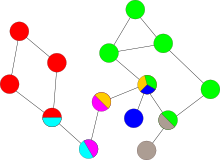
\includegraphics[]{imgs/bicomp.png}
    \end{center}
    Construct a tree of bi-connected components of the graph. Some of the approaches related to this structure needs you to do some updates in the parent of the node.

    The application is a problem with a lot of queries each query will give 3 vertices $a$,$b$ and $c$ and ask if there is a path that goes from $a$ to $b$, without passing in $c$. The answer is no if $a  == b$, $a == c$ or $c$ is an articulation point and is in the path of the block cut tree going from $a$ to $b$. The build is $\mathcal{O}(N)$, it gives you a tree, and you what you want from it.
    \inputwithhash{./solutions/Graph/block_cut_tree.cpp}

    \subsection{Two Edge Connected Components}
    Decompose the graph in Components connected by at least two edges. Can be used to create a tree as well, a "block cut" decomposition, but with edges instead of vertices.

    \inputwithhash{./solutions/Graph/2cc.cpp}

\chapter{Trees}
      \section{Dicas}
    \begin{itemize}
    \item A menor quantidade de arestas que você precisa adicionar em uma árvore para que não exista mais pontes é $\left \lceil \frac{qtd(folhas)}{2} \right \rceil$. Roda o DFS a partir de um cara que não é folha, ordena as folhas pelo tempo de entrada e cria uma aresta entre a folha $i$ e a folha $i + \frac{qtd}{2}$. Suponha que exista uma aresta que ainda é ponte, temos dois casos se considerarmos as folhas abaixo dessa aresta:
        \begin{itemize}
        \item Tem menos que $\frac{qtd}{2}$ folhas, assim com certeza uma dessas folhas vai ter uma aresta com uma folha de fora dessa "subárvore";
        \item Tem mais que $\frac{qtd}{2}$ folhas, com certeza essas folhas pertencem a primeira ou segunda metade do vetor de folhas ordenadas pelo tempo de entrada.
        \end{itemize}
    \end{itemize}

  
    \section{Diameter}
    Finding the diameter of the tree. Just do two DFS's, where in the first one you find the fatherst guy you can reach, and then find the other guy starting from the one you found before.
    \inputwithhash{./solutions/Tree/diameter.cpp}

      
    \section{LCA}
    A way to find the lowest common ancestor of two vertex $(a,b)$ in a tree. You can use binary lifting or you can store the depths of each vertex and finding the LCA is finding the node between $a$ and $b$ with minimum depth.
    \inputwithhash{./solutions/Tree/lca.cpp}

  
    
    \section{Euler tour tree}
    Euler tour é uma maneira de representar uma árvore usando o tempo de entrada e saída de cada nó para transformá-la em um vetor. Você pode usá-lo de 2 maneiras:
    \begin{itemize}
        \item Colocando o valor de um nó no tempo de entrada \texttt{tin} e não colocar nada no tempo de saída \texttt{tout}. Assim você pode fazer queries em subárvores.
        \item Colocar o valor de um nó no tempo de entrada \texttt{tin} e colocar o inverso do valor no tempo de saída \texttt{tout}. Se você realizar queries em caminhos que você entra e sai, a contribuição desse nó é cancelada. Para fazer a query de um path $u\rightarrow v$, você faz query da raiz para $u$, da raiz para $v$ e excluir $2$ vezes a query da raiz para $\text{lca}(u,v)$.
    \end{itemize}

      
    \section{Small to Large}
    Você quer juntar vários conjuntos disjuntos, se você realizar a união dos conjuntos sempre movendo os elementos do menor conjunto para o maior conjunto. No final a complexidade vai ser $\mathcal{O}(N\log(N))$. Para fazer o processo de \texttt{merge}, podemos usar a função \texttt{swap} do \texttt{STL}, a função realiza a troca em $\mathcal{O}(1)$ (é só trocar ponteiros), mas em algumas estruturas usar \texttt{swap} não é $\mathcal{O}(1)$. Mas você pode usar \texttt{a.swap(b)}, isso é $\mathcal{O}(1)$ para a maiorias das estruturas (um exemplo de estrutura que não é $\mathcal{O}(1)$ é o \texttt{array}). A implementação pode ser usando \texttt{DSU}.


\subsection{Small to Large com HLD Trick}
Ao fazer o Small to Large em uma árvore, você pode realizar a decomposição da árvore em arestas leves e pesadas, daí para cada vértice não vamos fazer o Small to Large normalmente, vamos adotar uma abordagem para a aresta pesada e outra para as arestas leves. Para a aresta pesada, vamos reaproveitar a resposta dela, para as arestas leves, vamos recuperar os vértices quando atravessamos as arestas leves e calcular a contribuição desses vértices em $\mathcal{O}(N)$. Isso não fica lento, pois para a abordagem bruteforce das arestas leves, cada vértice vai ser considerado no máximo $\log(N)$ vezes, pois cada vértice só aparece na abordagem bruteforce para cada ancestral que ele é ligado por uma aresta leve, mas no caminho da raiz para o vértice vão existir no máximo $\log(N)$ arestas leves.

A ideia dessa abordagem é não fazer o merge dos grupos do DSU e aí evitar uma possível complexidade que deixa a união dos grupos mais lento. Tipo no problema Distinct Colors do Cses que desse jeito não precisamos usar \texttt{map}/\texttt{set} para realizar a união dos grupos.

\inputwithhash{./solutions/DataStructures/DSU_HLD.cpp}

      
    \section{HLD}
    Dado uma árvore você quer responder perguntas sobre caminhos e também ser capaz de atualizar valores na árvore, vamos dividir a árvores em caminhos pesados e fazer uma \texttt{Seg} pra cada caminho.
    
    \inputwithhash{./solutions/Tree/hld.cpp}

  
    \section{Centroid Decomposition}
    Uma forma de aplicar divisão e conquista em árvores, escolhemos um centroide da árvore e dividimos a árvore a partir desse centroide e achamos os centroides das outras subárvores. Para problemas de centroide, vamos querer fazer, em geral, duas coisas:
    \begin{itemize}
        \item Fazer computações durante a construção do centroide, cada centroide representa um conjunto de caminhos do total de caminhos existentes da árvore. Daí podemos resolver problemas sobre caminhos.
        \item Fazer a decomposição em centroides da árvore e resolver o problema em cima dessa nova árvore.
    \end{itemize}

    Existem algumas propriedades importantes sobre a decomposição em centroides:
    \begin{itemize}
        \item A árvore vai ter profundidade igual a $\log_2(N)$;
        \item Para todo par de vértices $u$,$v$, se $L$ é o menor ancestral comum de $u$ e $v$ na decomposição em centroides, então o caminho de $u$ para $v$ na árvore original pode ser visto como o caminho de $u$ para $L$ e de $L$ para $v$, ou seja, $L$ está no caminho simples de $u$ para $v$.
        \item Qualquer um dos $\frac{n\cdot(n-1)}{2}$ caminhos possíveis na árvore original passa por um centroide.
    \end{itemize}

    \inputwithhash{./solutions/Tree/centroid.cpp}

    Exemplo 1: Dado uma árvore com $n$ nós, o objetivo é contar o número de caminhos distintos que contém exatamente $k$ arestas.

    \inputwithhash{./solutions/Tree/FixedLengthPathsI.cpp}
    
    Exemplo 2: Temos uma árvore com $n$ nós, cada nó pode ter duas cores, azul ou vermelho. Inicialmente o nó $1$ é vermelho e todos os outros são da cor azul, nós vamos fazer dois tipos de queries:
    \begin{itemize}
        \item Pintar um nó azul de vermelho;
        \item Calcular a menor distância para um nó vermelho a partir de um nó $u$.
    \end{itemize}

    \inputwithhash{./solutions/Tree/xenia&tree.cpp}

      
    
    \section{Tree Isomorphism}
    Geramos um id para cada árvore, também podemos fazer isso para subárvore. O \texttt{r[]} são as raízes arbitrárias que criamos, podemos passar uma raiz da árvore, mas se queremos comparar árvores que não estão enraizadas, usamos os centroides da árvore como raiz para comparar.

    \inputwithhash{./solutions/Tree/treehash.cpp}

  
    \section{Virtual Tree}
    A different way to approach trees problems. Main idea here is to create a tree with the "relevant nodes". Normally related to colors and problems which we solve looking for each color at a time.
    
    \inputwithhash{./solutions/Tree/virtual_tree.cpp}

      
    
    \section{Link Cut Tree}
    A link cut tree is a data structure that uses splay trees to represent a forest of rooted trees and can perform the following operations with an amortized upper bound time complexity of $\mathcal{O}(\log N)$:
    \begin{itemize}
        \item Linking a tree with a node by making the root of the tree a child of any node of another tree
        \item Deleting the edge between a node and its parent, detaching the node's subtree to make a new tree
        \item Find the root of the tree that a node belongs to
    \end{itemize}

    These operations all use the $\texttt{access}(v)$ subroutine,
which creates a preferred path from the root of the represented tree to vertex $v$, making a corresponding auxiliary splay tree with $v$ as the root.

    \inputwithhash{./solutions/Tree/linkcut.cpp}

\chapter{Geometry}
      \section{Dicas}
    \begin{itemize}
        \item Trick de rotacionar o plano em 45° graus no sentido horário transformando as coordenadas de $(x,y)$ para $(x+y,y-x)$. Depois dessa transformação, a Manhattan Distance vira a Chebyshev Distance (dado dois pontos $(x_1,y_1)$ e $(x_2,y_2)$, a distância é $\max(|x_1-x_2|,|y_1-y_2|)$). Além disso, as coordenadas são dilatadas por $\sqrt{2}$.
    \end{itemize}

  
    \section{Simple Geometry}
    This section will have alot of functions used in geometry problems. They are related to points, lines, circles and polygons.
    \subsection{Points, Lines and Polygons}
    This is the base of all codes in geometry. u can change the type from ldb to ll and also change the EPS. The rest is pretty much fixed.
    \inputwithhash{./solutions/Geometry/geobase.cpp}
    \subsection{Circles}
    This section will have alot of algorithms related to circles and their description.

    A tangent to a circle is a line in the plane of a circle which intersects the circle in exactly one point. This point is called the point of tangency.

    A tangent of two circles is a common internal tangent if the intersection of the tangent and the line segment joining the centers is not empty.

    \begin{center}
    \begin{minipage}{.5\textwidth}
    \centering
    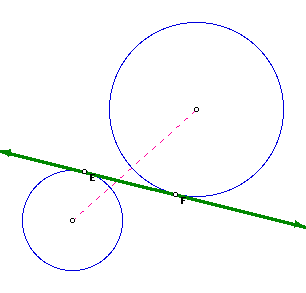
\includegraphics[scale = 0.5]{imgs/internal1.png}
    \end{minipage}%
    \begin{minipage}{0.5\textwidth}
    \centering
    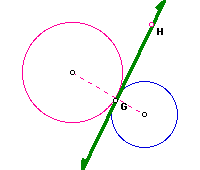
\includegraphics[scale = 0.5]{imgs/internal2.png}
    \end{minipage}
    \end{center}
    
    
    A tangent of two circles is a common external tangent if the intersection of the tangent and the line segment joining the centers is empty.

    
    \begin{center}
    \begin{minipage}{.5\textwidth}
    \centering
    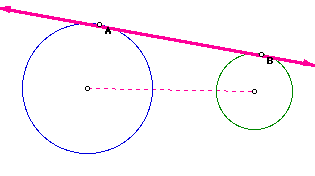
\includegraphics[scale = 0.5]{imgs/external1.png}
    \end{minipage}%
    \begin{minipage}{0.5\textwidth}
    \centering
    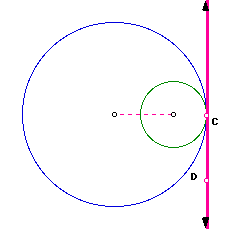
\includegraphics[scale = 0.5]{imgs/external2.png}
    \end{minipage}
    \end{center}

    The CircumCenter of a triangle is the minimum enclosing circle of a triangle. We can also calculated the minimum enclosing circle of a polygon.

    \begin{center}
    \begin{minipage}{.3\textwidth}
    \centering
    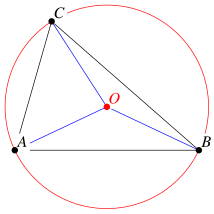
\includegraphics{imgs/circumcenter.png}
    \end{minipage}%
    \begin{minipage}{0.7\textwidth}
    \centering
    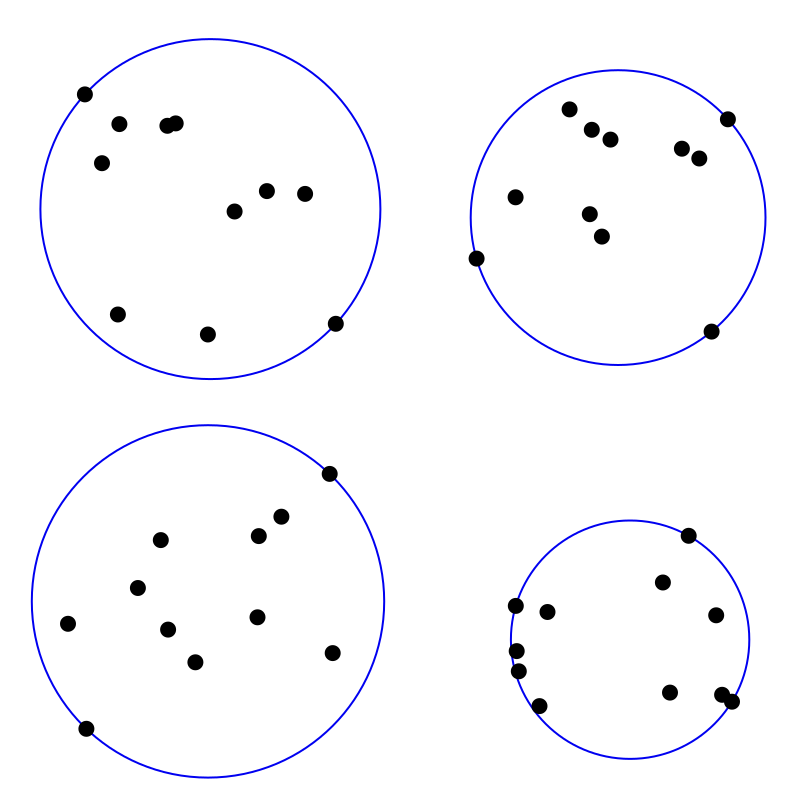
\includegraphics[scale = 0.5]{imgs/mec.png}
    \end{minipage}
    \end{center}

    \inputwithhash{./solutions/Geometry/circle.cpp}

  
    \section{Convex Hull}
        \subsection{Rotation Calipers}
        Diameter from a convex Polygon.
        
        Solution $O(n)$. Original Problem (NCPC 2013 - D).
        
        \ \\
        
        \begin{tabular}{|p{31cm}|}
          \begin{verbatim}
            Implementacao do Convex Hull do CP-ALGORITHMS
            Para usar crie um vetor com os pontos,
            		vector<pt> pts;
            e execute
            		convex_hull(|pts|);
            Apos isso, o vector pts sera alterado e ele so tera os pontos do Convex Hull 
            na ordem horaria, comecando do elemento de menor x, como segunda condicao menor y.
            
            Como funciona o algoritmo
            - Acha os dois extremos de x.
            - Monta dois subgrupos, os "up" e os "down", em relacao
            Convex Hull na parte superior e inferior.
            - Itera pelos pontos e usa o produto vetorial para ver se
            ele forma um sentido horario, se formar adiciona.
            - Remove todos os anteriores ao ultimo ponto adicionado que agora, com o ponto
            atual, formando um sentido anti-horario
            \end{verbatim}
        \end{tabular}
        \\
        
        \inputwithhash{./solutions/Geometry/MaxDistanceBetweenPoints.cpp}

          
    \section{Line Sweep}
        \subsection{Points Inside Triangles}
        Given $n$ triangles with vertices {($x_i$, $y_i$), ($x_i + d$, $y_i$), ($x_i$, $y_i + d$)}, and $q$ points, compute for each triangle, the number of points that lie inside or in boundary of him. $O(nlogn)$. (Original Problem: CODECHEF - TRIANGULAR QUERIES)
        \inputwithhash{./solutions/Geometry/PointsInsideTriangles.cpp}
        \newpage
        \subsection{Ranking Problem}
        Given $n$ students that attended to $3$ contests, and all of them have different ranks, between $1$ and $n$ inclusive, for each contest. We say that one student $a$ is better that student $b$, if all ranks of student $a$ in each contest is lesser that student $b$. A student is said to be excellent if no other student is better than him. How many excelent students there exists ?
        
        This solutions runs in $O(nlogn)$. (Original Problem: SPOJ: NICEDAY)
        
        \inputwithhash{./solutions/Geometry/RankingProblem.cpp}
        \newpage
        \subsection{Balls Falls and Segments}
        Given $n$ segments (non horizontal and with no common points), and $m$ balls in a 2D plane, say for each ball the x point which he falls. (This solution was upload, the source code is just for only one ball, but the overall complexity is still $O(nlogn)$ if the number of balls is $O(n)$).
        
        This solutions runs in $O(nlogn)$. Original Problem (NCPC 2013 - H).
        
        \inputwithhash{./solutions/Geometry/WaterFalls.cpp}
        \newpage
        \subsection{Checking Points Inside Convex Polygon}
            % \subsubsection{Offline}
            % Given $n$ points in 2D plane, and a Convex Polygon, check for each of these $n$ points, if them are strict inside or not of polygon.
            
            % This solutions runs in $O(nlogn)$ but i used Fracion Class to Take Care with double error precisions, so the overall solution in this case is $O(nlogn^2)$.
            
            % \lstinputlisting{./solutions/Geometry/PointsInsideConvexPolygon.cpp}
            % \newpage
            \subsubsection{Online}
            Given one point and a Convex Polygon, with vertices in counter clockwise order, check if this point is inside or in boundary of him.
            
            This solutions runs in $O(logn)$.
            
            \inputwithhash{./solutions/Geometry/PointsInsideConvexPolygonOn.cpp}
        % \newpage
        % \subsection{Area of Rectangles Union}
        % Given a set of N axis aligned rectangles, you need to find the area of their union. Each rectangle is represented by two points, one lower-left point and one upper-right point. The coordinates are all integers.
        
        % This solutions runs in $O(nlogn)$. Original Problem (HackerEarth - Line Sweep Tutorial, Sample Exercicise)
        
        % \lstinputlisting{./solutions/Geometry/RectangleUnion.cpp}
        % \newpage
        \subsection{Radial Sweep}
        You are given $N$ red points and $M$ blue points on a 2D plane.

        You are required to delete the minimum number of points(the deleted points can be of both colors) so that it's possible to draw a line such that all remaining red points are on one side of the line while all remaining blue points are on the other side of the line.
        
        This solutions runs in $O(n^2logn)$. Original Problem (Codechef, REDBLUE - DEC17)
        
        \inputwithhash{./solutions/Geometry/RadialSweep.cpp}
        \subsection{Radial Sweep sem Double}
        You are in a point inside a square NxN. There are some rocks(polygons) inside the square, u need to discover how many points form the perimeter of the square, are visible, form your oirigin
    
        In this problem, there are three types of events: when our ray hits a fence point, enters a rock, or exits a rock.

    The second and third types of events can be found for each rock by sorting the rays to its vertices by bearing and then taking the two endpoints of the sorted list. These two rays are the two tangents to the rock.
    
    We can then perform a radial sweep to find the fence posts that Farmer Don can see - these fence posts are simply the ones where the number of type-2 and type-3 events we've processed so far are equal.
        
        \inputwithhash{./solutions/Geometry/SeeingTheBoundary.cpp}
    % \newpage

      \section{Minimum Perimeter Triangle}
    Given $n$ points in a 2D plane, return the minimum perimeter that can be formed taking three points, collinear points are allowed. $O(nlogn)$. (Original Problem - Google Code Jam WF 2009 - B)
    \inputwithhash{./solutions/Geometry/MinPerimeterTriangle.cpp}
    % \section{Line Sweep}

\chapter{Miscellaneous}
      \section{Game Theory}
        Vamos nos importar com os jogos imparciais com dois jogadores, ou seja, jogos em que os movimentos disponíveis e a vitória/derrota depende apenas do estado do jogo. Em outras palavras, a única diferença entre os dois jogadores é que um deles se move primeiro. Além disso, assumimos que o jogo são de informação perfeita, ou seja, não existe informação que é escondida dos jogadores (os jogadores sabem as regras e os possíveis movimentos), assim os jogadores sempre podem tomar decisões ótimas. Assume-se que o jogo é finito, depois de um certo número de movimentos, algum dos jogadores vai estar em um estado perdedor, e sempre alguém perde e alguém ganha. 
        
        Esses jogos podem ser vistos como grafos direcionados acíclicos, os vértices são estados e as arestas são movimentos. Um vértice com grau de saída zero é um vértice perdedor (o jogador que tiver que fazer um movimento nesse estado perde).

        Um estado perdedor é aquele que todos os movimentos levam a um estado vencedor para o outro jogador e um estado vencedor é aquele em que existe ao menos uma transição para um estado perdedor.

        \subsection{Jogo de Nim}
        Qualquer jogo imparcial pode ser reduzido a um jogo de Nim (jogo das pilhas de pedras). Nesse jogo o estado é determinado de acordo com o xor das quantidades das pilhas de pedras que temos, se o xor é zero, o estado é perdedor, se o xor é diferente de zero, o estado é vencedor.
        \subsection{Teorema de Sprague-Grundy}
        Vamos reduzir cada estado do jogo a um estado do jogo de Nim, mais especificamente cada estado do jogo original pode ser mapeado para um jogo de Nim com uma pilha de tamanho $x$. O número $x$ é chamado de valor de Grundy ou valor-nim do estado. Além disso, esse número pode ser calculado da seguinte maneira:

        \[
        x = \text{mex} \ \{x_1, \dots, x_k \}
        \]

        Onde $x_i$ é o valor de Grundy para todo os próximos estados a partir do estado atual (vértices que o estado atual pode transitar para). Vendo o jogo como um grafo, podemos calcular o valores de Grundy começando dos vértices com grau de saída igual a zero. Assim os estados vencedores são aqueles diferentes de zero, e os perdedores são os iguais a zero, assim como no jogo de Nim.

        A ideia é que os estados perdedores são jogos de Nim que não tem nenhuma pedra, e nesses estados, o mex é igual a zero, pois eles são vistos como vértices sem grau de saída. Os outros estados (vértices), tem estados alcançáveis, e esses estados só podem ser alcançados ao realizar um movimento, como estamos reduzindo o jogo a um jogo de Nim, temos que tirar ou colocar uma quantidade de pedras. Então a partir do valor atual (que representa uma pilha de pedras) temos que conseguir gerar todos os valores adjacentes, e o valor que resume isso é o mex dos valores adjacentes. Uma vez que a partir do mex, conseguimos gerar todos os valores menores que o mex tirando alguma quantidade de pedras, e conseguimos gerar todos os valores maiores, colocando alguma quantidade de pedras. 
        
        Mas uma pergunta seria, porque o valor de Grundy não pode ser qualquer outro valor? Ele não pode ser um valor maior que o mex, porque se fosse, esse estado teria que conseguir gerar o estado com o mex tirando alguma quantidade de pedras, mas esse estado não existe (porque se existisse o mex não seria o mex). Ele não pode ser menor também, porquê significa que estamos realizando um movimento em que tiramos nenhuma pedra (movimentar para o vértice que tem mesmo valor de Grundy que o meu), mas isso não pode acontecer no jogo de Nim.

        Para calcular o número de Grundy, fazemos:
        \begin{itemize}
            \item Obter todas as possíveis transições a partir do estado atual;
            \item Cada transição pode levar a um conjunto independente de jogos, calculamos o valor de Grundy para cada jogo de maneira independente e depois fazemos o xor-sum deles, uma vez que cada jogo é uma pilha do jogo de Nim.
            \item Depois de calcular os valores de Grundy para cada transição, calculamos o estado atual como o \text{mex} desses números.
        \end{itemize}

        \subsection{Dicas}
        \begin{itemize}
            \item \textit{Teoria do Espelhamento}: Se o seu oponente pode espelhar todas as suas ações, este é um estado de derrota.
            \item Podem existir ciclos modulares, vale brutar.
            \item Em algum momento pode se tornar sempre win, ou sempre loss.
            \item Se a gente transformar o problema num nim, podemos usar o teorema de grundy, que basicamente é achar os casos derrota + fazer o mex.
        \end{itemize}
        
        Example 1: There is a heap of $n$ coins and two players who move alternately. On each move, a player chooses a heap and divides into two nonempty heaps that have a different number of coins. The player who makes the last move wins the game. Here for big N the answer is always first.

        
    \inputwithhash{./solutions/Miscellaneous/GrundyGame.cpp}

        Example 2: There is a staircase consisting of $n$ stairs, numbered $1,2,\ldots,n$. Initially, each stair has some number of balls. There are two players who move alternately. On each move, a player chooses a stair $k$ where $k\neq1$ and it has at least one ball. Then, the player moves any number of balls from stair $k$ to stair $k-1$. The player who moves last wins the game. Here, every odd position is losing, u can see them as "dark holes", using the "Teoria do Espelhamento", so it's just N/2 Nim games.

        
    \inputwithhash{./solutions/Miscellaneous/StairGame.cpp}

    \subsection{Nim Multiplication}
        A 2D NIM Game int the form of NXM can be reduced
        to the Nim Multiplication of 2 1D NIM GAMES
        in the form of NimMult(Grundy(N),Grundy(M))
        
        \inputwithhash{./solutions/Miscellaneous/NimMult.cpp}

  \section{Binary Search}
    \subsection{Parallel Binary Search}
    (Original Problem: Atcoder Grand Contest 2 D)
     \inputwithhash{./solutions/Miscellaneous/agc002_d.cpp}
% \section{Next\_Permutation - C++}
%     \lstinputlisting{./solutions/Miscellaneous/next_permutation.cpp}

  \section{Big Num}
    Implementação de Big Number em C++.
        \inputwithhash{./solutions/Miscellaneous/bignum.cpp}
    \subsection{D\&C for Multiplyng two big numbers}
        \inputwithhash{./solutions/Miscellaneous/karatsuba.cpp}

  
\section{Fractions}
    Implementação de frações em C++.
        \inputwithhash{./solutions/Miscellaneous/fractions.cpp}

  

\section{Bitsets}
Some $O(N^2)$ solutions can be optimized using bitsets. Mainly knapsack problems.
An important point is to use the "popcount" optimization  in target of pragma.

how to initialize:

\begin{lstlisting}
bitset<size> variable_name;
bitset<size> variable_name(DECIMAL_NUMBER);
bitset<size> variable_name("BINARY_STRING")
\end{lstlisting}

Every position can be accessed as a vector, also size must be constant. We get an constant optimization of 32. every bit operation used in integers can be used in bitsets.

Some functions in bitsets:
\begin{center}
\begin{tabular}{ c | l }
  set()  & Set the bit value at all bitset to 1.  \\ 
 reset() & Set the bit value at all bitset to 0.  \\  
 flip() & Flip the bit value at all bitset.\\
 set(idx) & Set the bit value at the given idx to 1.  \\ 
 reset(idx) & Set the bit value at a given idx to 0.  \\  
 flip(idx) & Flip the bit value at the given idx.\\
 count() & Count the quantity of bits set.\\  
 any() & Checks if any bit is set.\\
 all() & Check if all bit is set.\\
 none() & Checks if none bit is set.\\
 size() & Returns the size of the bitset.\\
 to\_string() & Converts bitset to std::string.\\
 to\_ulong() & Converts bitset to unsigned long.\\
 to\_ullong() & Converts bitset to unsigned long long.\\
 \_Find\_first() & return index of first bit set. \\
 \_Find\_next(idx) & return index of first bit set after idx.
\end{tabular}
\end{center}

  
\section{Built in functions}

Some Built in functions in GCC(remember that if u are using ll, need to add ll at the end):
\begin{center}
\begin{tabular}{ c | l }
  \_\_builtin\_popcount(x)  & Counts the quantity of one’s(set bits) in an integer.  \\ 
 \_\_builtin\_parity(x) & Checks the Parity of a integer.\\
 
 &Returns true(1) if odd parity(odd quantity of set bits)\\
 
 & Returns false(0) for even parity(even quantity of set bits).  \\  
 \_\_builtin\_clz(x) &  Counts the leading quantity of zeros of the integer.\\
 \_\_builtin\_ctz(x) & Counts the trailing quantity of zeros of the integer.  \\ 
 \_\_builtin\_popcountll(x)  & Counts the quantity of one’s(set bits) in an long long.  \\ 
 \_\_builtin\_parityll(x) & Checks the Parity of a long long.\\
 
 &Returns true(1) if odd parity(odd quantity of set bits)\\
 
 & Returns false(0) for even parity(even quantity of set bits).  \\   
 \_\_builtin\_clzll(x) &  Counts the leading quantity of zeros of the long long.\\
 \_\_builtin\_ctzll(x) & Counts the trailing quantity of zeros of the long long.  \\ 
\end{tabular}
\end{center}
clz can be used to find the first set bit, since u can use:
\begin{lstlisting}
int x;
ll xl;
int fsi =  31 - __builtin_clz(x);
int fsll = 63 - __builtin_clzll(xl);
\end{lstlisting}

  \section{Priority Queue and Set Comparators}

Set Comparators
Operator Overloading:
\begin{lstlisting}
#include <bits/stdc++.h>
using namespace std;

struct Edge {
	int a, b, w;
	bool operator<(const Edge &y) const { return w < y.w; }
};

int main() {
	int M = 4;
	set<Edge> v;
	for (int i = 0; i < M; ++i) {
		int a, b, w;
		cin >> a >> b >> w;
		v.insert({a, b, w});
	}
	for (Edge e : v) cout << e.a << " " << e.b << " " << e.w << "\n";
}
\end{lstlisting}
Functors:

\begin{lstlisting}
#include <bits/stdc++.h>
using namespace std;

struct Edge {
	int a, b, w;
};

struct cmp {
	bool operator()(const Edge &x, const Edge &y) const { return x.w < y.w; }
};

int main() {
	int M = 4;
	set<Edge, cmp> v;
	for (int i = 0; i < M; ++i) {
		int a, b, w;
		cin >> a >> b >> w;
		v.insert({a, b, w});
	}
	for (Edge e : v) cout << e.a << " " << e.b << " " << e.w << "\n";
}
\end{lstlisting}

Functors can also be used in priority queues, but needs vector as a container:

\begin{lstlisting}
priority_queue<int, vector<int>, cmp> c; 
\end{lstlisting}
Built in Functors:
\begin{lstlisting}
set<int, greater<int>> a; //max set
map<int, string, greater<int>> b; // max map
priority_queue<int, vector<int>, greater<int>> c; // min heap
\end{lstlisting}

  \section{Lambda Expressions}
Basic Lambda Syntax
    A lambda expression consists of the following:
\begin{center}
    [capture list] (parameter list) {function body}
\end{center}
The capture list and parameter list can be empty, so the following is a valid lambda:
\begin{lstlisting}
[](){cout << "Hello, world!" << endl;}
auto func1 = [](int i) {cout << ":" << i << ":";};
func1(x);
\end{lstlisting}
Using \& in capture list it will have access to the scope.

Recursive lambda using function:
\begin{lstlisting}
int main() {
	function<int(int, int)> gcd = [&](int a, int b) {
		return b == 0 ? a : gcd(b, a % b);
	};
	cout << gcd(20, 30) << '\n';  // outputs 10
}
\end{lstlisting}

      
\section{Fast input output}
        \inputwithhash{./solutions/Miscellaneous/IOPT.cpp}

  \section{Trick for faster Unordered Map}
        \inputwithhash{./solutions/Miscellaneous/umap.cpp}

  \section{Faster Hash Table}
    \inputwithhash{./solutions/Miscellaneous/hashtablerobada.cpp}

  \section{StringStream}
    A way to parse strings in c++.
    \inputwithhash{./solutions/Miscellaneous/stringstream.cpp}

  \section{Karmarkar-Karp}
    Heuristic algorithm to divide a set in two others set, in the way that the difference between the sum of this two new sets will be minimal.
    The error of this heuristc algorithm is $\mathcal{O}(n^{-lg(n)})=\mathcal{O}(\frac{1}{n^{lg(n)}})$
    \inputwithhash{./solutions/Miscellaneous/karmakarp.cpp}

\chapter{Problemas}
  
\section{Minimizar quantidade de grupos sem elementos repetidos}
%https://codeforces.com/problemset/problem/2022/B
Dado $N$ elementos distintos, com o elemento $i$ aparecendo $A_i$ vezes. Queremos formar grupos de tamanho máximo $K$, tal que cada grupo não pode conter elementos repetidos e todos os elementos devem pertencer a um grupo. Qual o menor número de grupos que temos que formar?

Podemos resolver esse problema em $\mathcal{O}(N)$, a solução é calcular $\max\left\{\max\{A_1,A_2,\dots,A_N\}, \left\lceil \frac{\sum A_i}{K} \right\rceil  \right\}$.

Vamos chamar a menor quantidade de grupos de $qt_{min}$, $qt_{min}$ tem dois lower bounds importantes, $qt_{min} \ge \max\left\{ A_1,A_2,\dots,A_N \right\}$, pois não podemos repetir elementos em um mesmo grupo. Além disso, com certeza $qt_{min} \ge \left\lceil \frac{\sum A_i}{K} \right\rceil$, uma vez que cada grupo pode ter no máximo tamanho $K$, então temos que ter no mínimo $\left\lceil \frac{\sum A_i}{K} \right\rceil$ grupos. Então a resposta é no mínimo $\max\left\{\max\{A_1,A_2,\dots,A_N\}, \left\lceil \frac{\sum A_i}{K} \right\rceil  \right\}$. Agora basta provarmos que sempre conseguimos uma configuração com $qt_{min}$ grupos, a prova é bem simples. Podemos imaginar que cada grupo é uma linha de uma matriz, assim temos uma matriz $qt_{min} \times K$, conseguimos pra cada coluna colocar colocar todos os elementos (uma vez que $qt_{min} \ge \max\left\{ A_1,A_2,\dots,A_N \right\}$), assim é só de maneira gulosa colocar os elementos de um mesmo grupo numa mesma coluna e preencher a matriz dessa maneira.

Tem um outro jeito recursivo de construir os grupos que é interessante, mas para facilitar vamos considerar que $K = 2$. Suponha que um elemento $x$ apareça tal que $2 \cdot A_x = N$, nesse caso pareamos todos os outros elementos com o $x$.  Agora suponha que para todos os elementos $2 \cdot A_x < N$, então vamos escolher aleatoriamente dois elementos e parear eles, daí $N$ vai para $N-2$ e como o dobro de todas as quantidades são menores que $N$, então vale que $2 \cdot A_x <= N-2$.

\inputwithhash{./solutions/Problemas/KarSalesman.cpp}

  
\section{Maximizar área de uma matriz em que todas as células são válidas}
%https://codeforces.com/group/btcK4I5D5f/contest/623901/problem/L
Dado uma matriz $N\times M$, cada célula pode ser válida ou inválida, qual a maior área que contém só células válidas?

Podemos resolver esse problema em $\mathcal{O}(N \times M)$, a ideia da solução é manter para cada linha qual o maior segmento contíguos de células válidas e daí iterar nas colunas e considerar pra cada linha a partir da coluna, que essa linha é um "limitante" para uma sub-matriz que contem essa linha. E manter as linhas mais acima da atual que tem tamanho maior ou igual a linha atual.

Vamos pré-calcular alguns valores, pra cada célula $(i,j)$ vamos calcular $dist(i,j)$ que é o tamanho da sequência começando em $(i,j)$ que só contém células válidas, conseguimos calcular isso em $\mathcal{O}(N \times M)$. Agora vamos calcular para cada célula $(i,j)$, dois valores $acima(i,j)$ e $abaixo(i,j)$, tal que $acima(i,j)$ é a linha $X$ mais acima de tal modo que $\displaystyle \min_{X \le k \le i}\{dist(k,j)\} = dist(i,j)$, o $abaixo(i,j)$ é a linha mais abaixo que obedece a mesma restrição. Para calcular isso podemos iterar pelas colunas e iterar nas linhas e calcular o cara mais distante com valor maior ou igual a linha atual usando esquema com \texttt{stack}. Depois de calcular esses valores, podemos iterar pelas células e verificar os valores de $acima(i,j)$ e $abaixo(i,j)$ e calcular $ans = \max\{ans, dist(i,j) \cdot (abaixo(i,j) - acima(i,j) + 1)\}$. Um adendo é que não precisamos fazer uma matriz para $acima$ e $abaixo$, podemos só fazer um vetor que representa a uma coluna e daí calculamos pra cada coluna e já calculamos a resposta pra essa coluna.

\inputwithhash{./solutions/Problemas/MaxAreaMatriz.cpp}

  
\section{Quantidade mínima de movimentos com restrição de vida}
%https://codeforces.com/problemset/problem/2149/F
Um herói com $H$ pontos de vida começa no ponto $0$ e quer alcançar o ponto $D$, para alcançá-lo, ele pode realizar duas operações:
\begin{itemize}
    \item Descansar e aumentar a vida em $1$ ponto;
    \item Mover uma posição para frente.
\end{itemize}
A cada movimento (alterar a posição atual), a vida do herói é decrementada, se o movimento é o $i$-ésimo consecutivo, então a vida vai cair em $i$ pontos. A cada movimento, a vida do heróis deve ser maior que $0$, qual a quantidade mínima de operações para o herói alcançar $D$? Como exemplo de operações, considere que $H = 7$ e $D = 4$, então uma sequência de operações poderiam ser:
\begin{enumerate}
    \item Mover de $0$ para $1$ e perder $1$ de vida;
    \item Mover de $1$ para $2$ e perder $2$ de vida;
    \item Mover de $2$ para $3$ e perder $3$ de vida;
    \item Descansar e ganhar $1$ de vida;
    \item Mover de $3$ para $4$ e perder $1$ de vida.
\end{enumerate}

Podemos resolver esse problema em $\mathcal{O}(\log(N))$, a solução é fazer uma busca binária na quantidade de dias que o herói vai descansar, e dado uma quantidade $X$ de descansos, verificar se é possível chegar no ponto $D$ sem nunca ter $H \le 0$. Para verificar se vai der certo é verificar se $r_1 \cdot PA\left(\lfloor\frac{D}{X+1}\rfloor + 1\right) + r_2 \cdot PA\left(\lfloor\frac{D}{X+1}\rfloor\right) < H + X$, tal que $r_1 = D\% (X+1)$ (resto da divisão), $r_2 = (X+1) - r_1$ e $PA(X) = \sum_{i=1}^X i$.

O mínimo de operações para chegar em $D$ é igual a $D$, que seria apenas realizar $D$ movimentos para frente, então o que vai ``piorar'' a resposta são os descansos. Vamos supor que você vai ter $X$ descansos, vamos ver se é possível saber se com esses $X$ descansos conseguimos chegar ao final de tal modo que $H > 0$ em todo momento. Vamos considerar a configuração que perdemos menos vida, essa configuração vai ser colocar os descansos em posições uniformes, então vamos ter intervalos contíguos de tamanho mais ou menos igual de operações de movimentos, para cada intervalo vamos perder $PA(TAM)$ de vida tal que $TAM$ é o tamanho do intervalo.

Vamos calcular o custo dessa configuração, se temos $X$ descansos, vamos ter $X+1$ intervalos contíguos de movimentos para frente. Desses intervalos, $r_1 = D\%(X+1)$ intervalos vão ter tamanho $\lfloor\frac{D}{X+1}\rfloor+1$ e $r_2 = (X+1) - r_1$ vão ter tamanho $\lfloor\frac{D}{X+1}\rfloor$, assim, vamos perder $r_1 \cdot PA\left(\lfloor\frac{D}{X+1}\rfloor + 1\right) + r_2 \cdot PA\left(\lfloor\frac{D}{X+1}\rfloor\right)$ pontos de vida na melhor configuração. Uma afirmação é dizer que só conseguimos chegar a $D$ com $X$ descansos se minimamente nossa vida máxima é maior que o quanto de vida perdemos, ou seja, $r_1 \cdot PA\left(\lfloor\frac{D}{X+1}\rfloor + 1\right) + r_2 \cdot PA\left(\lfloor\frac{D}{X+1}\rfloor\right) < H + X$. Porque, caso contrário, qualquer configuração $S$, vai ter custo maior ou igual ao custo ideal, e temos que chegar no final com valor maior que $0$, assim o custo tem que ser menor que o máximo de vida que é $H + X$.

Outra afirmação é que se $r_1 \cdot PA\left(\lfloor\frac{D}{X+1}\rfloor + 1\right) + r_2 \cdot PA\left(\lfloor\frac{D}{X+1}\rfloor\right) < H + X$, então a configuração uniforme vai dar certo, ou seja, em todo momento $H > 0$. Mas o que garante que não existe um momento em que a vida é menor ou igual a $0$, mesmo que a desigualdade seja verdade? Suponha que numa configuração a vida chegue a um valor menor ou igual a $0$ e isso aconteça num ponto $P$, com certeza é impossível chegar no ponto $D$ com uma vida maior que zero, pois seria necessário que o saldo de vida entre $P+1$ e $D$, seja positivo, mas isso é impossível, pois colocando os descansos em pontos uniformes, qualquer sufixo começando em $D$ vai ter saldo menor ou igual a $0$. Assim, se a desigualdade vale, é impossível em qualquer ponto a vida estar menor ou igual a $0$.

\inputwithhash{./solutions/Problemas/NezukointheClearing.cpp}

  
\section{Minimizar o custo da configuração de uma matriz dado restrições de linhas e colunas}
%https://codeforces.com/gym/105677/problem/J
Considere uma matriz $N\times M$ composta por células pretas e brancas em que cada célula preta é representada pelo número $0$ e cada célula branca por um número no intervalo fechado de $[1,9]$. Temos dois tipos de restrições, a restrição horizontal e vertical, as duas restrições são aplicáveis somente para as células pretas. A restrição horizontal é determinada pela tripla $(x,y,S)$ tal que $(x,y)$ representa a célula preta em que a restrição é aplicada e $S$ indica que as células brancas contíguas a direita de $(x,y)$ devem ter soma igual a $S$. A restrição horizontal é determinada também por uma tripla $(x,y,S)$ tal que $(x,y)$ representa a célula preta em que a restrição é aplicada e $S$ indica que as células brancas contíguas abaixo de $(x,y)$ devem ter soma igual a $S$. Dado uma matriz inicial e um conjunto de restrições, qual o custo mínimo para fazer com que a matriz obedeça a todas as restrições tal que o custo é igual a a diferença absoluta do valor de cada célula branca na matriz original pelo valor na nova matriz. Além disso, cada célula branca é coberta por exatamente uma restrição horizontal e uma vertical.

Podemos resolver esse problema em $\mathcal{O}(MCMF)$. Modelamos uma rede em que cada restrição horizontal e vertical são vértices, consideramos cada célula branca $W_i$ como uma aresta entre um par de restrições $R_i$ e $C_i$ (restrição linha e coluna respectivamente). Mas cada aresta vai ser considerada como dois vértices $W_i$, $W'_i$ ou $W_{in}$, $W_{out}$. Ligamos arestas do $Src$ para cada restrição $R_i$ com capacidade igual a $R_i.v'$ (valor da restrição modificada - vai ser esclarecido) e custo $0$, fazemos o mesmo tipo de aresta entre $Snk$ e $C_i$. Ligamos arestas com capacidade igual a infinito (esse infinito pode ser $8$) entre cada $R_i$ e $W_i$ correspondente, o análogo entre $W'_i$ e $C_i$. Além disso, ligamos duas arestas entre $W_i$ e $W'_i$, a primeira com capacidade $W_i.v-1$ e custo $-1$ e outra com capacidade $8 - (W_i.v-1)$ e custo $1$. Executamos o $MCMF$ e a resposta é possível somente se $\sum R_i.v' = \sum C_i.v' = Max\_Flow$ e o custo mínimo é $\sum (W_i.v -1) ~-~ Min\_Cost$.

Cada $W_i$ pode ser unicamente determinado por um par $(R_i,C_i)$ e $W_i$ contribui com o seu valor para as restrições horizontais e verticais. Assim, $\sum R_i.v = \sum W_i.v = \sum C_i.v$, então faz sentido pensar que a cada $1$ de valor de $W_i$, ele vai restringir em $1$ o valor do seu $R_i$ e $C_i$ correspondentes. A partir disso, podemos pensar em uma modelagem em que cada $W_i$ serve como uma aresta entre um $R_i$ e um $C_i$, porque passar fluxo em $W_i$ (passar valor em $W_i$) resulta em restringir o valor de $R_i$ e $C_i$. Por fim, consideramos uma modelagem em que cada $R_i$ tem uma aresta com $Src$ com capacidade igual ao seu valor, o análogo entre cada $C_i$ e $Snk$, além disso cada $W_i$ representa uma aresta que liga um $R_i$ e $C_i$. Existe uma consideração importante, parece correto dizer que a capacidade de $W_i$ é $9$, mas se considerarmos que é nove, temos a escolha de passar zero de fluxo por $W_i$ e essa escolha significa dizer que o valor de $W_i$ é zero, mas isso não pode ser possível, pois $W_i.v \in [1,9]$. Para contornar isso subtraímos $1$ de cada $W_i$, agora cada $R_i$ e $C_i$ vão ter um novo custo $c'$ tal que $c' = c - qtd_{W}$, ou seja, o novo custo de cada restrição é o custo original menos a quantidade de células brancas na restrição. Agora passar $0$ de fluxo representa colocar a célula com valor $1$, o intervalo $[1,9]$ mapeia para o intervalo $[0,8]$.

Essa modelagem serviria para verificar se existe alguma configuração que atende todas as restrições, mas não calcula o custo mínimo. Vamos aplicar um custo para cada aresta, as arestas do tipo $(Src,R_i)$ e $(C_i,Snk)$ vão ter custo $0$. Para cada aresta $W_i$, vamos criar dois vértices $W_i,W'_i$ e considerar arestas de $(R_i,W_i)$ e $(W'_i,C_i)$ com capacidade $8$ e custo $0$. Vamos também criar duas arestas de $W_i$ para $W'_i$, uma com capacidade $W_i.v'$ (subtrair $1$ de cada célula branca) e custo $-1$ e outra com capacidade $8-W_i.v'$ e custo $1$. A arestas principais são entre $W_i$ e $W'_i$, sempre que possível vamos passar o máximo de fluxo na aresta de custo $-1$ (queremos minimizar o custo, assim vamos querer saturar a aresta, ou seja, passar o valor original da célula). Se vamos passar mais fluxo que $W_i.v'$, temos que passar na aresta de custo $1$. Essa modelagem é genial porque para valores menores ou iguais a $W_i.v'$, sempre vamos querer passar o máximo de fluxo (porque o custo é negativo), mas para valores maiores que $W_i.v'$, vamos querer passar o mínimo de fluxo, assim o fluxo sempre vai convergir para passar o mais próximo possível de $W_i.v'$ e assim minimizando o custo. Mas por que essa modelagem vai dar o custo mínimo?

Considere uma configuração que atenda as restrições, nessa configuração vão existir células em que o novo valor é menor ou igual ao original (considere o valor original como $x$ e o novo como $x'$) e outras em que o novo valor é maior que o original (considere o valor original como $y$ e o novo com $y'$). Podemos dizer que $Custo = \sum(x - x') + \sum(y'-y)$, mas também podemos dizer que $Custo = \sum(x-x') + \sum(y'-y + (y-y)) = \sum(x-x') + \sum(y'-y) + \sum(y-y) = \sum(x+y) + \sum(y' - y) + \sum(-x')$. O termo $\sum(x+y)$ refere-se ao somatório do valor das células original que é constante, então minimizar $Custo$ equivale a minimizar $\sum(y' - y) + \sum(-x')$ e esse é exatamente a modelagem de custo da nossa rede. O termo $\sum(y'-y)$ equivale a saturar a aresta de custo negativo e passar uma quantidade de fluxo na aresta de custo $1$ e o termo $\sum(-x')$ é passar fluxo na aresta de custo $-1$. Assim a resposta vai ser $\sum W_i.v - Min\_Cost$.

\inputwithhash{./solutions/Problemas/RecoveringtheTablet.cpp}

  
\section{Minimizar soma de coordenadas com operação de ``inverter'' dois pontos em sequência}
%https://atcoder.jp/contests/arc189/tasks/arc189_b
Dado $N$ pontos com coordenadas inteiras distintas dispostos numa linha, é possível realizar uma operação: escolher um inteiro $i$ tal que $1 \le i \le N-3$ e, seja $M$ o ponto médio entre as posições do $i$-ésimo e $(i+3)$-ésimo pontos em ordem crescente de coordenadas, mova os $(i+1)$-ésimo e $(i+2)$-ésimo pontos para suas posições simétricas em relação a $M$. Faça as operações de modo a minimizar a soma das coordenadas dos $N$ pontos.

Podemos resolver esse problema em $\mathcal{O}(N \log(N))$, a ideia principal da solução é pensar nos pontos em termo da distância dele para o ponto anterior. Calculando essas distâncias, podemos ordená-las por um critério e usar essa ordenação para calcular a resposta.

Primeiro vamos determinar como uma operação realizada em $i$ altera os pontos $i+1$ e $i+2$. Considerando $X_i$ como a localização do $i$-ésimo ponto e $M$ como ponto médio de $X_i$ e $X_{i+3}$, temos duas situações de operação para $X_j$, ponto entre $X_i$ e $X_{i+3}$:
\begin{itemize}
    \item $X_j$ antes de $M$: $X_j \xrightarrow{op} (M-X_j)+M \rightarrow 2M-X_j$
    \item $X_j$ depois de $M$: $X_j \xrightarrow{op} M-(X_j-M) \rightarrow 2M-X_j$
\end{itemize}
Então independente da posição de $X_j$ em relação a $M$ sua nova posição é $2M - X_j = (X_i+X_{i+3})-X_j$. Assim a nova posição dos pontos vai ser:
\[
    \begin{cases}
    X_i &= X_i \\
    X_{i+1} &= X_{i+1} \\
    X_{i+2} &= X_{i+2} \\
    X_{i+3} &= X_{i+3}  
    \end{cases}
    \xrightarrow{op}
    \begin{cases}
    X'_i &= X_i \\
    X'_{i+1} &= (X_i+X_{i+3})-X_{i+2} \\
    X'_{i+2} &= (X_i+X_{i+3})-X_{i+1} \\
    X'_{i+3} &= X_{i+3} 
    \end{cases}
\]

Vamos mudar a forma como representamos os pontos, considerando $d_j = X_j - X_{j-1}$, vamos representar os pontos como $X_i = \sum_{j=1}^id_j = X_{i-1} + d_i$ (considere $X_0 = 0$). Ou seja, vamos representar um ponto usando a distância dele para os pontos anteriores, vamos olhar essas distâncias realizando a operação:
\[
    \begin{cases}
    X_i &= X_{i-1}+d_i \\
    X_{i+1} &= X_i+d_{i+1} \\
    X_{i+2} &= X_{i+1}+d_{i+2} \\
    X_{i+3} &= X_{i+2}+d_{i+3}  
    \end{cases}
    \xrightarrow{op}
    \begin{cases}
    X'_i     &= X'_{i-1}+d'_i \\
    X'_{i+1} &= X'_i+d'_{i+1} \\
    X'_{i+2} &= X'_{i+1}+d'_{i+2} \\
    X'_{i+3} &= X'_{i+2}+d'_{i+3}
    \end{cases}
    \rightarrow
    \begin{cases}
    d'_i     &= X'_i - X'_{i-1} \\
    d'_{i+1} &= X'_{i+1} - X'_i \\
    d'_{i+2} &= X'_{i+2} - X'_{i+1} \\
    d'_{i+3} &= X'_{i+3} - X'_{i+2}
    \end{cases}
    \rightarrow
\]
\[
    \begin{cases}
    d'_i     &= X_i - X_{i-1} \\
    d'_{i+1} &= (X_i+X_{i+3}-X_{i+2}) - X_i \\
    d'_{i+2} &= (X_i+X_{i+3}-X_{i+1}) - (X_i+X_{i+3}-X_{i+2}) \\
    d'_{i+3} &= X_{i+3} - (X_i+X_{i+3}-X_{i+1})
    \end{cases}
    \rightarrow
    \begin{cases}
    d'_i     &= d_i \\
    d'_{i+1} &= d_{i+3} \\
    d'_{i+2} &= d_{i+2} \\
    d'_{i+3} &= d_{i+1}
    \end{cases}
\]

Assim, realizar a operação troca as distâncias $d_{i+1}$ com $d_{i+3}$, ou seja, você só troca as distâncias de lugar. Além disso, essa troca só acontece com distâncias de mesma paridade, as distâncias que aparecem mais cedo, vai contribuir mais para o somatório, então ordenamos as distâncias e colocamos as menores primeiro.

\inputwithhash{./solutions/Problemas/MinimizeSum.cpp}

  
\section{Maximizar a soma de Manhattan Distances entre pares de pontos}
%https://codeforces.com/contest/2122/problem/C
Dado $2N$ pontos com coordenadas inteiras, escolha $N$ pares de ponto disjuntos $a_i$ e $b_i$ a fim de maximizar $\sum_{i=1}^N|X_{a_i} - X_{b_i}| + |Y_{a_i} - Y_{b_i}|$.

Podemos resolver esse problema em $\mathcal{O}(N\log(N))$, separamos cada ponto em 4 grupos de acordo com o índice do ponto se forem ordenados por $X$ e por $Y$ separadamente. Daí vamos colocar num mesmo par, os pontos que tem $X$ na metade menor e $Y$ na metade menor e os pontos que tem $X$ na metade maior e $Y$ na metade maior. E colocar num mesmo par, os pontos que tem $X$ na metade menor e $Y$ na metade maior e os pontos que tem $X$ na metade maior e $Y$ na metade menor.

A melhor configuração seria sempre tentar colocar um $X$,$Y$ pequenos com $X$,$Y$ grandes. Se ordenássemos os pontos em função de $X$ colocaríamos os índices na primeira metade com os da segunda metade, mas também, ao mesmo tempo, se ordenássemos em função de $Y$, os pontos da primeira metade ficariam com os da segunda metade. Mas fazer isso é possível?

Podemos classificar cada ponto em 4 grupos de acordo em qual metade cada ponto está quando ordenamos por $X$ e por $Y$.
\begin{table}[h]
    \centering
    \begin{tabular}{|c|c|c|}
    \hline
    \textbf{Grupo} & \textbf{Ordenação por $X$} & \textbf{Ordenação por $Y$} \\ \hline
    $A$ & Metade menor & Metade menor \\ \hline
    $B$ & Metade maior & Metade maior \\ \hline
    $C$ & Metade menor & Metade maior \\ \hline
    $D$ & Metade maior & Metade menor \\ \hline
    \end{tabular}
\end{table} \\
Vamos tentar colocar no mesmo par os caras do grupo $A$ com os caras de $B$, e colocar os caras do grupo $C$ com os caras de $D$. Mas para isso é necessário que $|A| = |B|$ e $|C| = |D|$, mas temos que:
\[
\begin{cases}
    |A| + |C| = N ~~(1)\\
    |A| + |D| = N ~~(2)\\
    |B| + |C| = N ~~(3)\\
    |B| + |D| = N ~~(4)
\end{cases} \xrightarrow[\text{subtraindo}~(4)~\text{de}~(2)]{\text{subtraindo}~(2)~\text{de}~(1)}
\begin{cases}
    |C|-|D| = 0 ~~(1)-(2) \\
    |A|-|B| = 0 ~~(2)-(4)
\end{cases} \rightarrow
\begin{cases}
    |C| = |D| ~~(1)-(2) \\
    |A| = |B| ~~(2)-(4)
\end{cases}
\]
Assim, sempre é possível parear $A$ com $B$ e $C$ com $D$.

\inputwithhash{./solutions/Problemas/ManhattanPairs.cpp}

\end{document}

% Para adicionar:
% github.com/felipesabino1/questoes_boas/DP/Bitmask/Matrix Exponentiation
% github.com/felipesabino1/questoes_boas/DP/Probability and Combinatorics/Pin some Element/ Cycles (Difficult).cpp
% Problema de LP com Bellman Ford
% Mo em arvore
